\chapter{Event Selection}

\begin{section}{Baseline selection}

One of the main challenges for a SUSY search is that the ratio of SM-to-SUSY events is $\mathcal{O}(10^{12} - 10^{14})$.
To surmount this problem, it is paramount to develop highly efficient signal-to-background discriminators.
Fortunately, SUSY signatures typically have characteristics unlike most SM processes.
For the T1tbs process, in particular, events are expected to have a large number of jets, many of which are b-quark jets, resulting in a large amount of \HT and many b-tagged jets.
Additionally, the mass scale of the event is expected to be larger than most SM events due to the high masses of the gluinos ($\mathcal{O}(1~\TeV)$), as discussed in Section~\ref{subsec:MJ}.

These features are used to construct the ``baseline selection'', defined as a basic set of requirements that events must pass, and to reduce the background-to-signal ratio to a more manageable value of $\mathcal{O}(10^2)$.
Here the baseline selection is defined as \baseNleps, \baseHT, \baseMJ, \baseNjets, and \baseNb.
To see the separation of signal and background in these variables, the corresponding ``N-1'' distributions, i.e. the distribution of a variable with the baseline selection applied except for the requirement corresponding to the binned variable, are depicted in Figure~\ref{fig:nminus1} with the black dashed vertical line representing the value of the baseline cut.
Additionally, a ``cutflow table'' that depicts the expected yields for background and signal processes as each baseline selection requirement is individually applied is shown in Table~\ref{tab:cutflow}.
Rows above the horizontal line correspond to requirements in the baseline selection, while those below correspond to additional kinematic cuts.

\begin{figure}[tbp!]
\centering
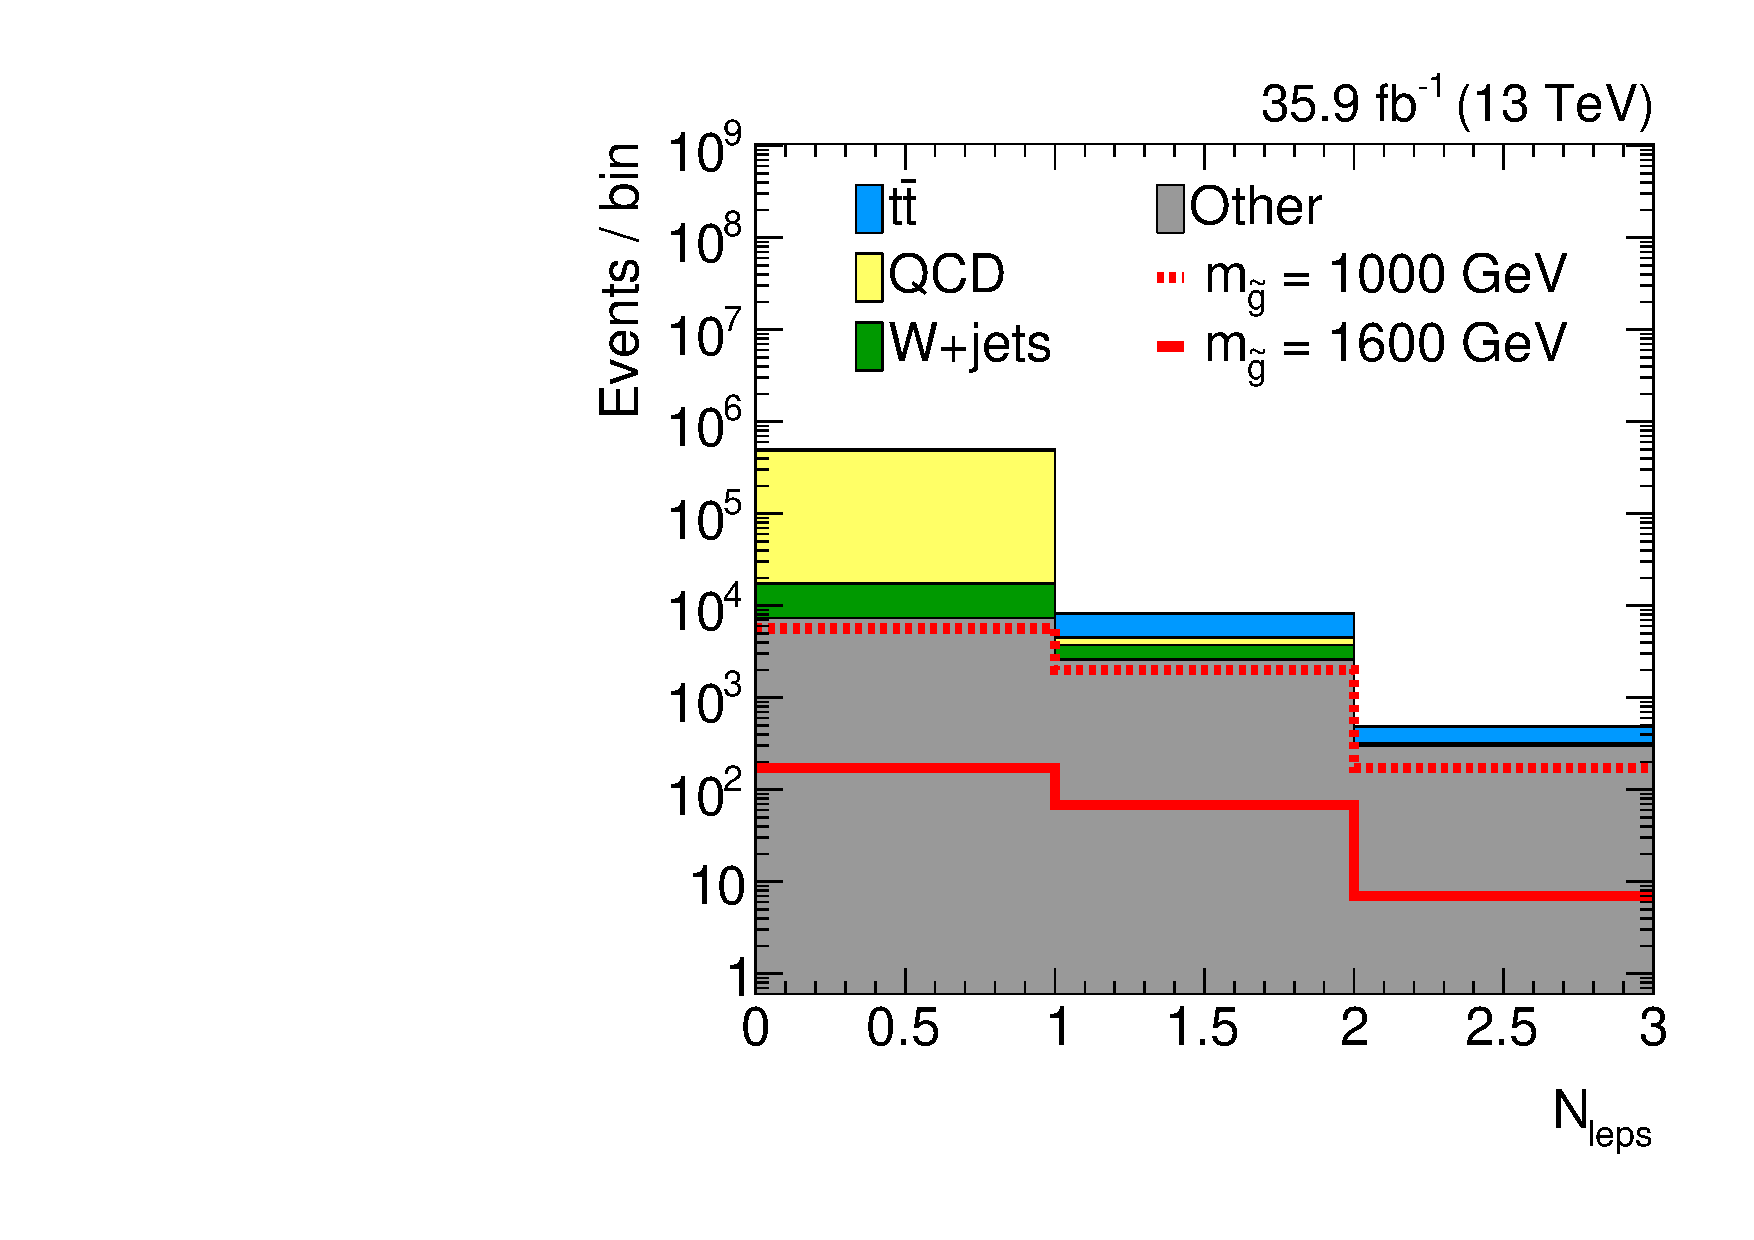
\includegraphics[angle=0,width=0.35\columnwidth]{fig/nminus1_nleps.pdf}
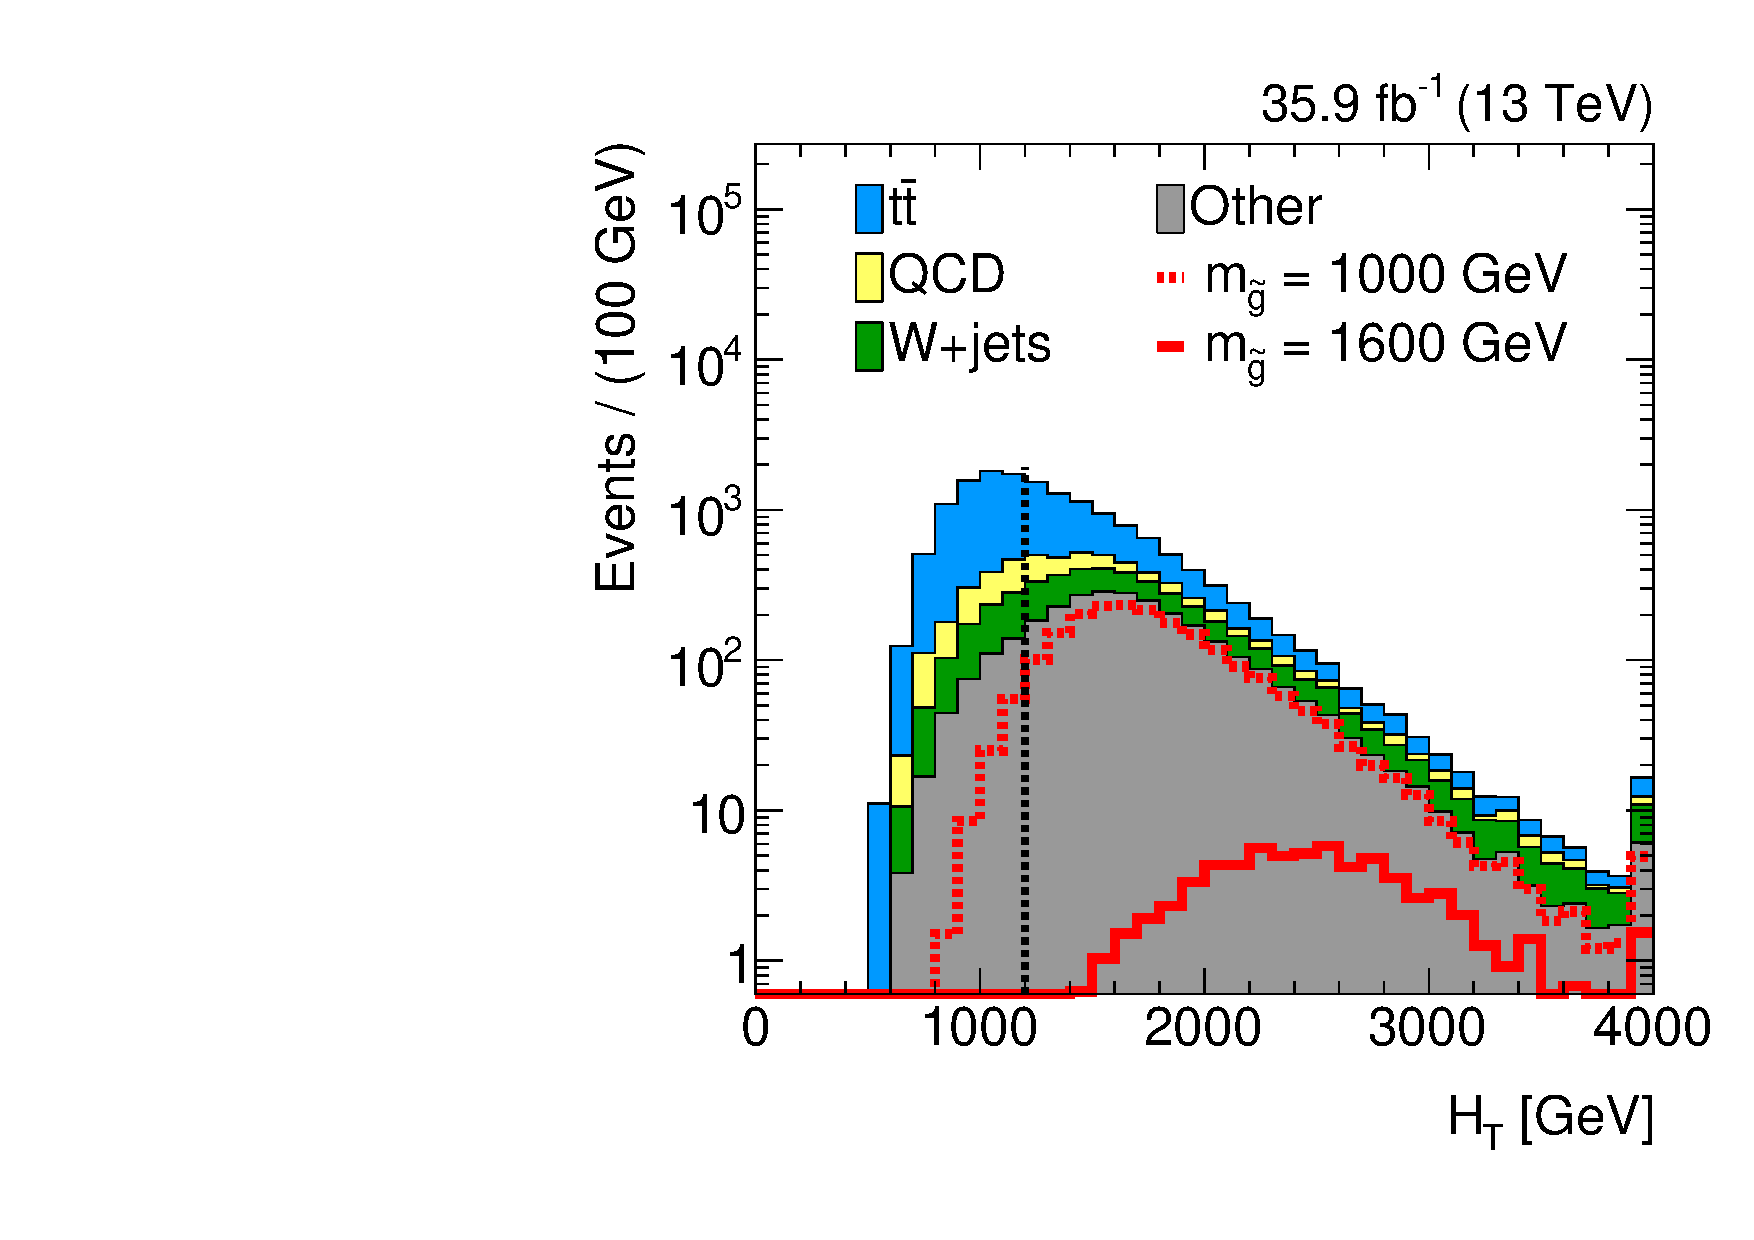
\includegraphics[angle=0,width=0.35\columnwidth]{fig/nminus1_ht.pdf}
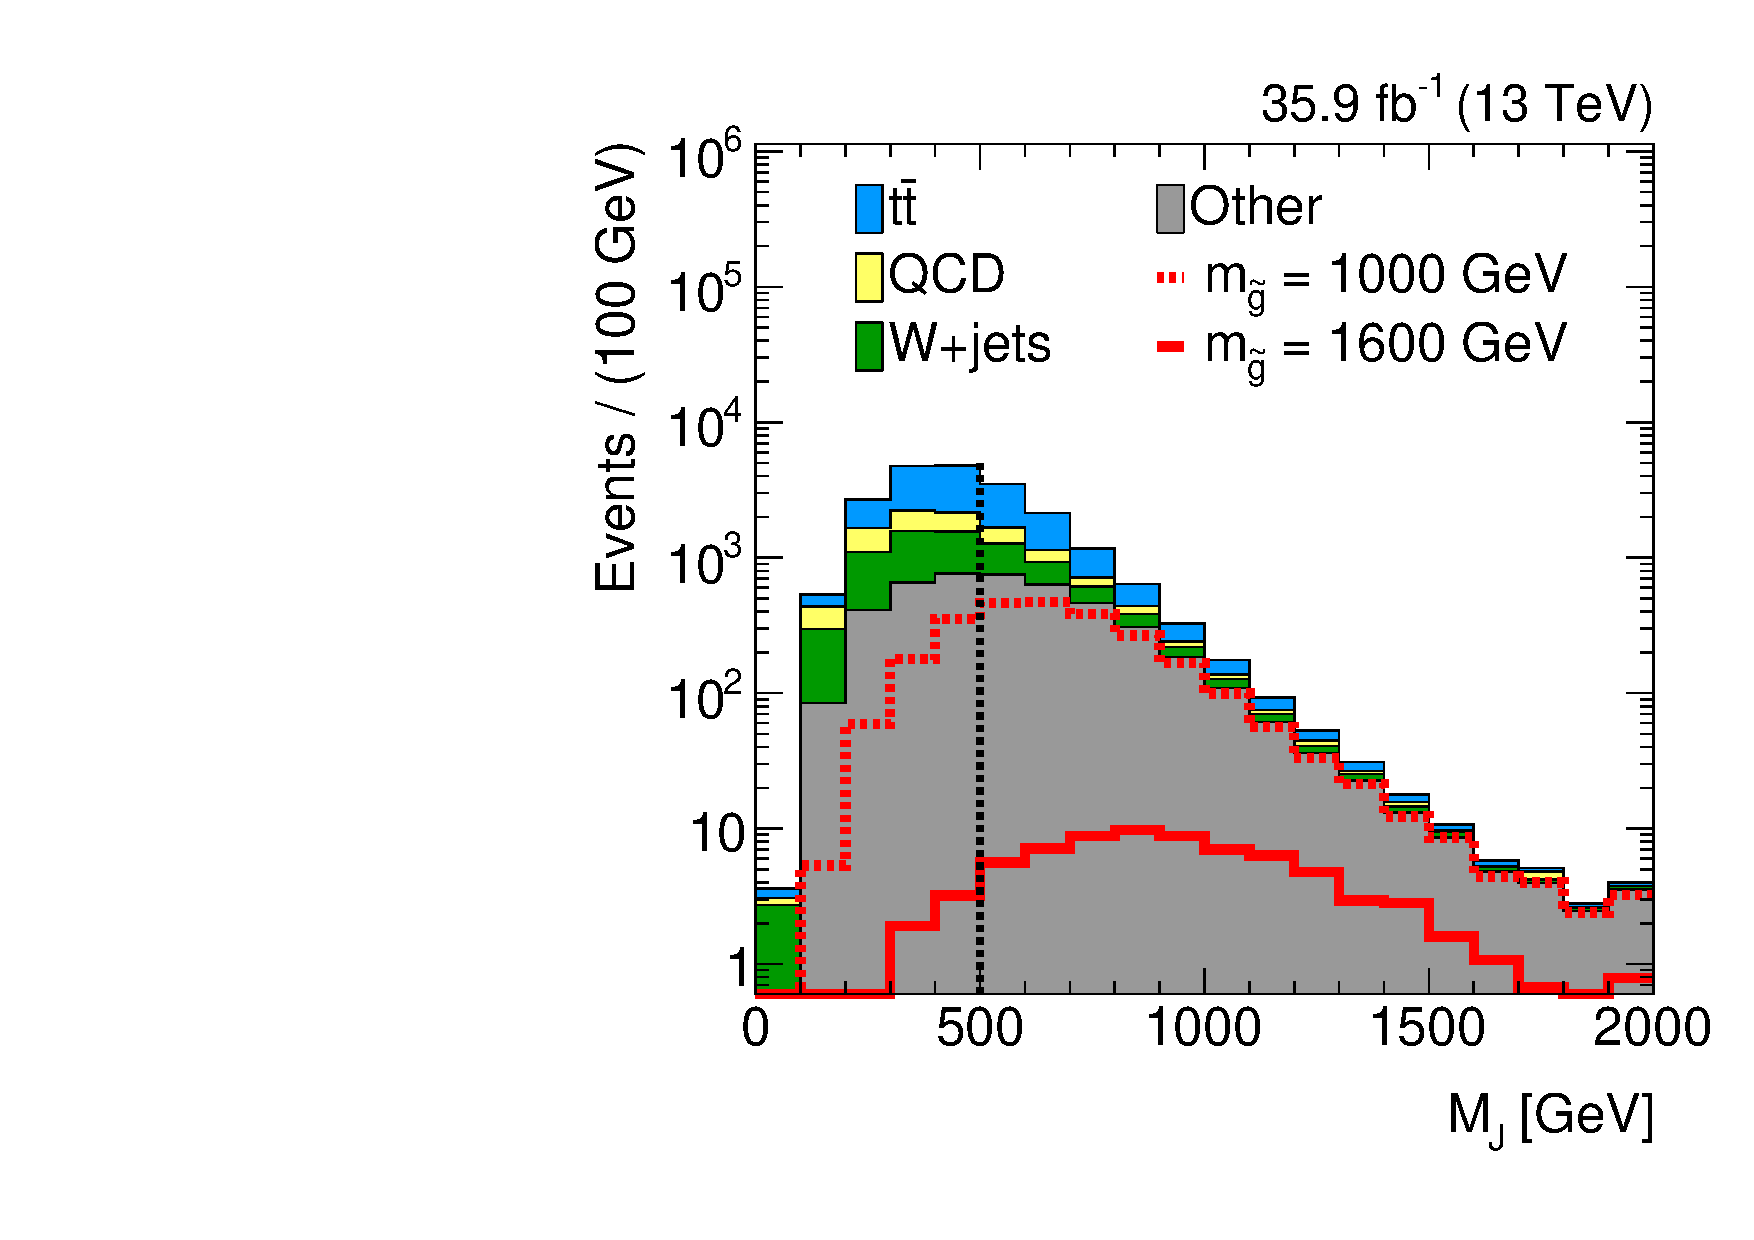
\includegraphics[angle=0,width=0.35\columnwidth]{fig/nminus1_mj.pdf}
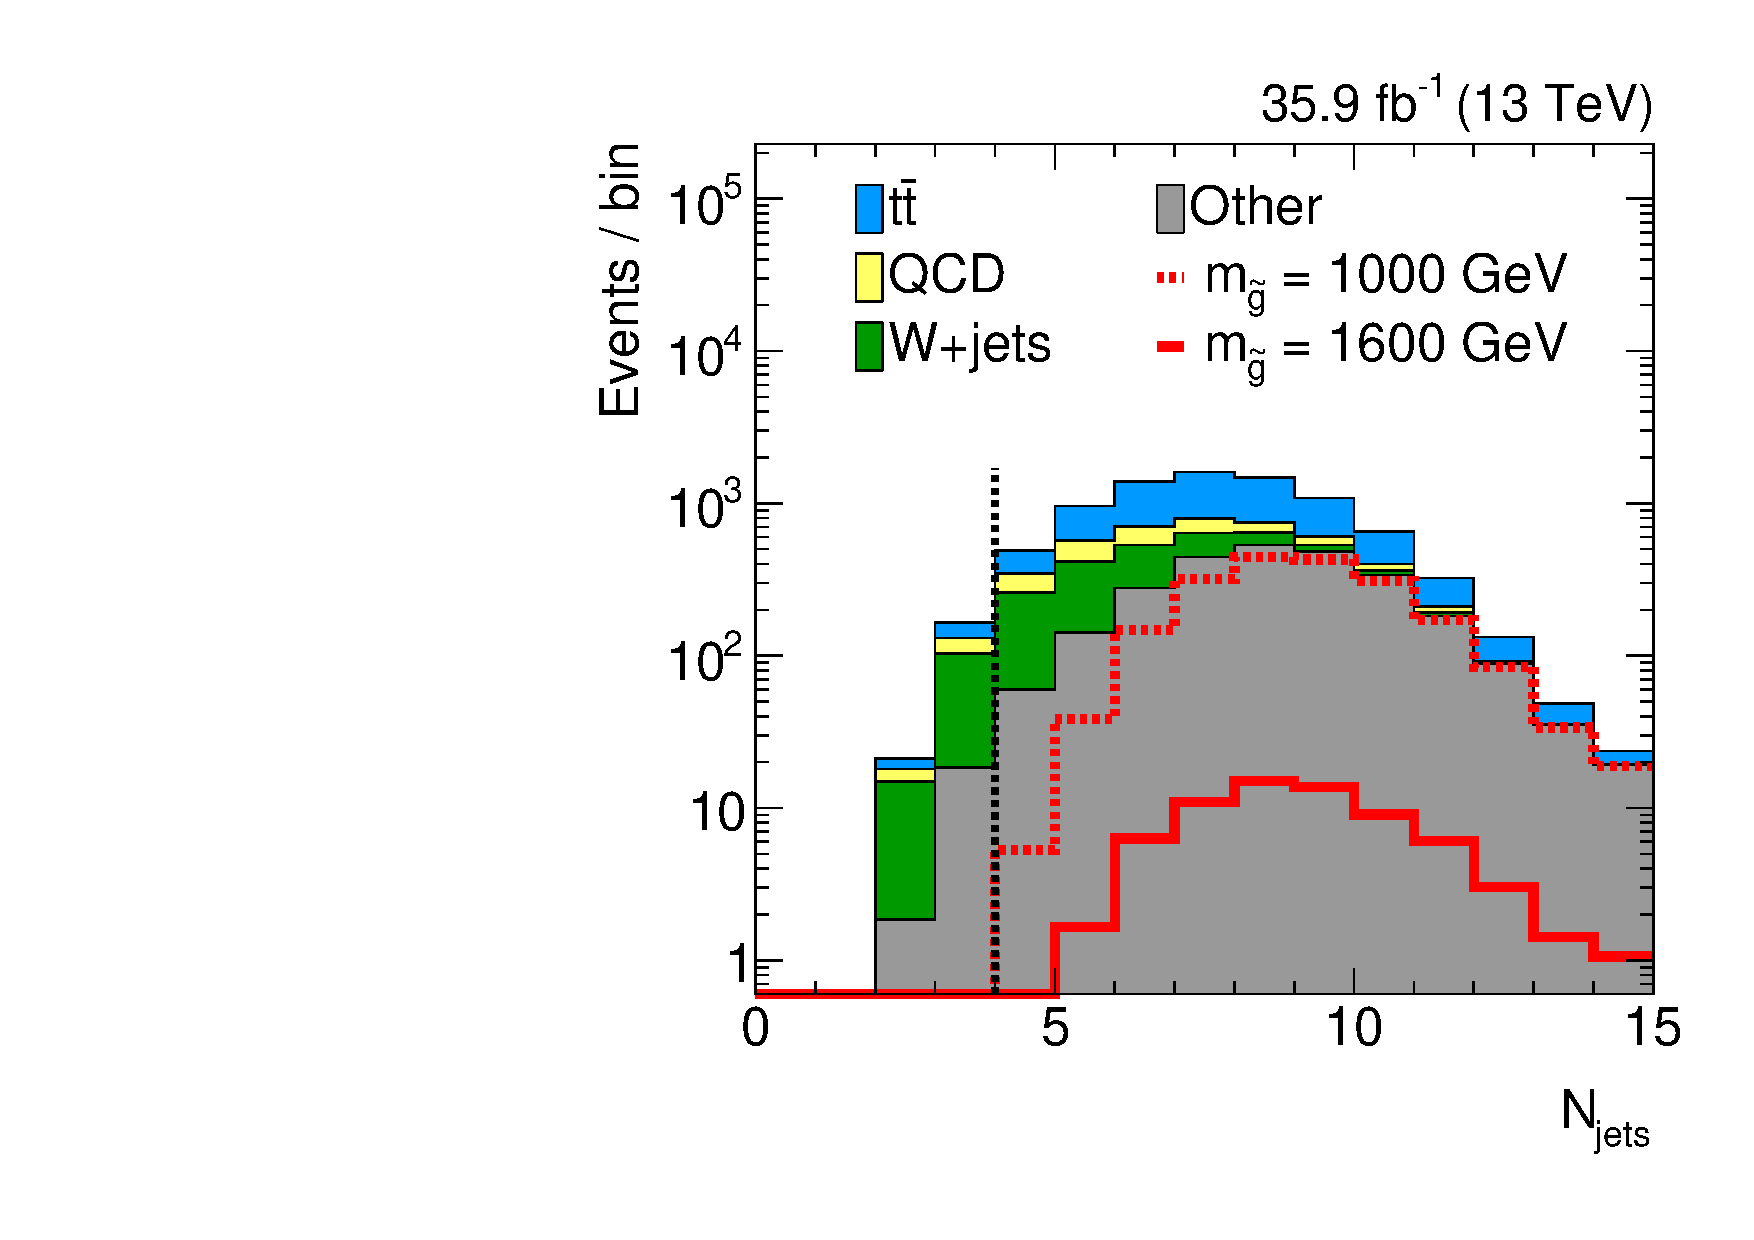
\includegraphics[angle=0,width=0.35\columnwidth]{fig/nminus1_njets.pdf}
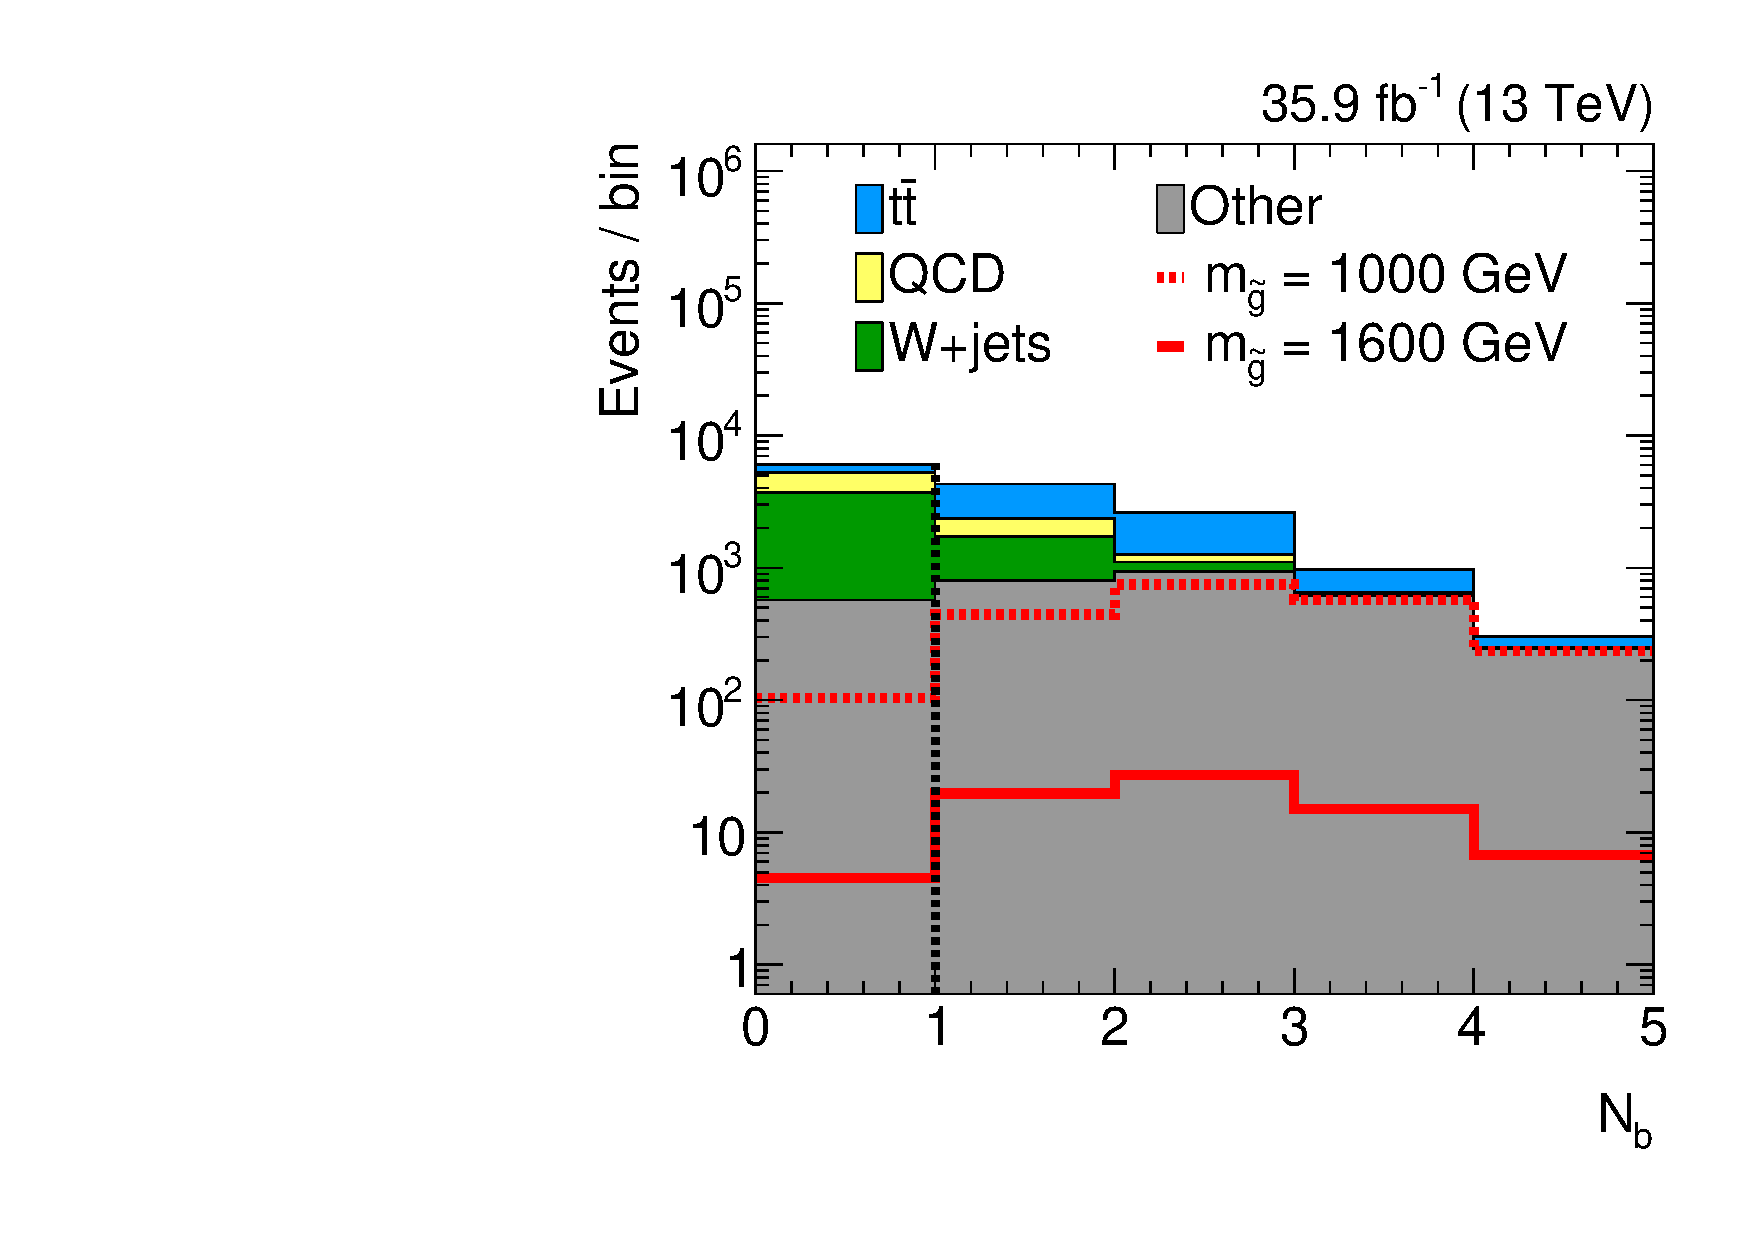
\includegraphics[angle=0,width=0.35\columnwidth]{fig/nminus1_nb.pdf}
\caption{The N-1 plots for \Nleps (top-left), \HT (top-right), \MJ (middle-left), \Njets (middle-right), and \Nb (bottom).
The black dashed vertical line represents the value of the corresponding baseline requirement.}
\label{fig:nminus1}
\end{figure}

\begin{table}[tbp!]
\centering
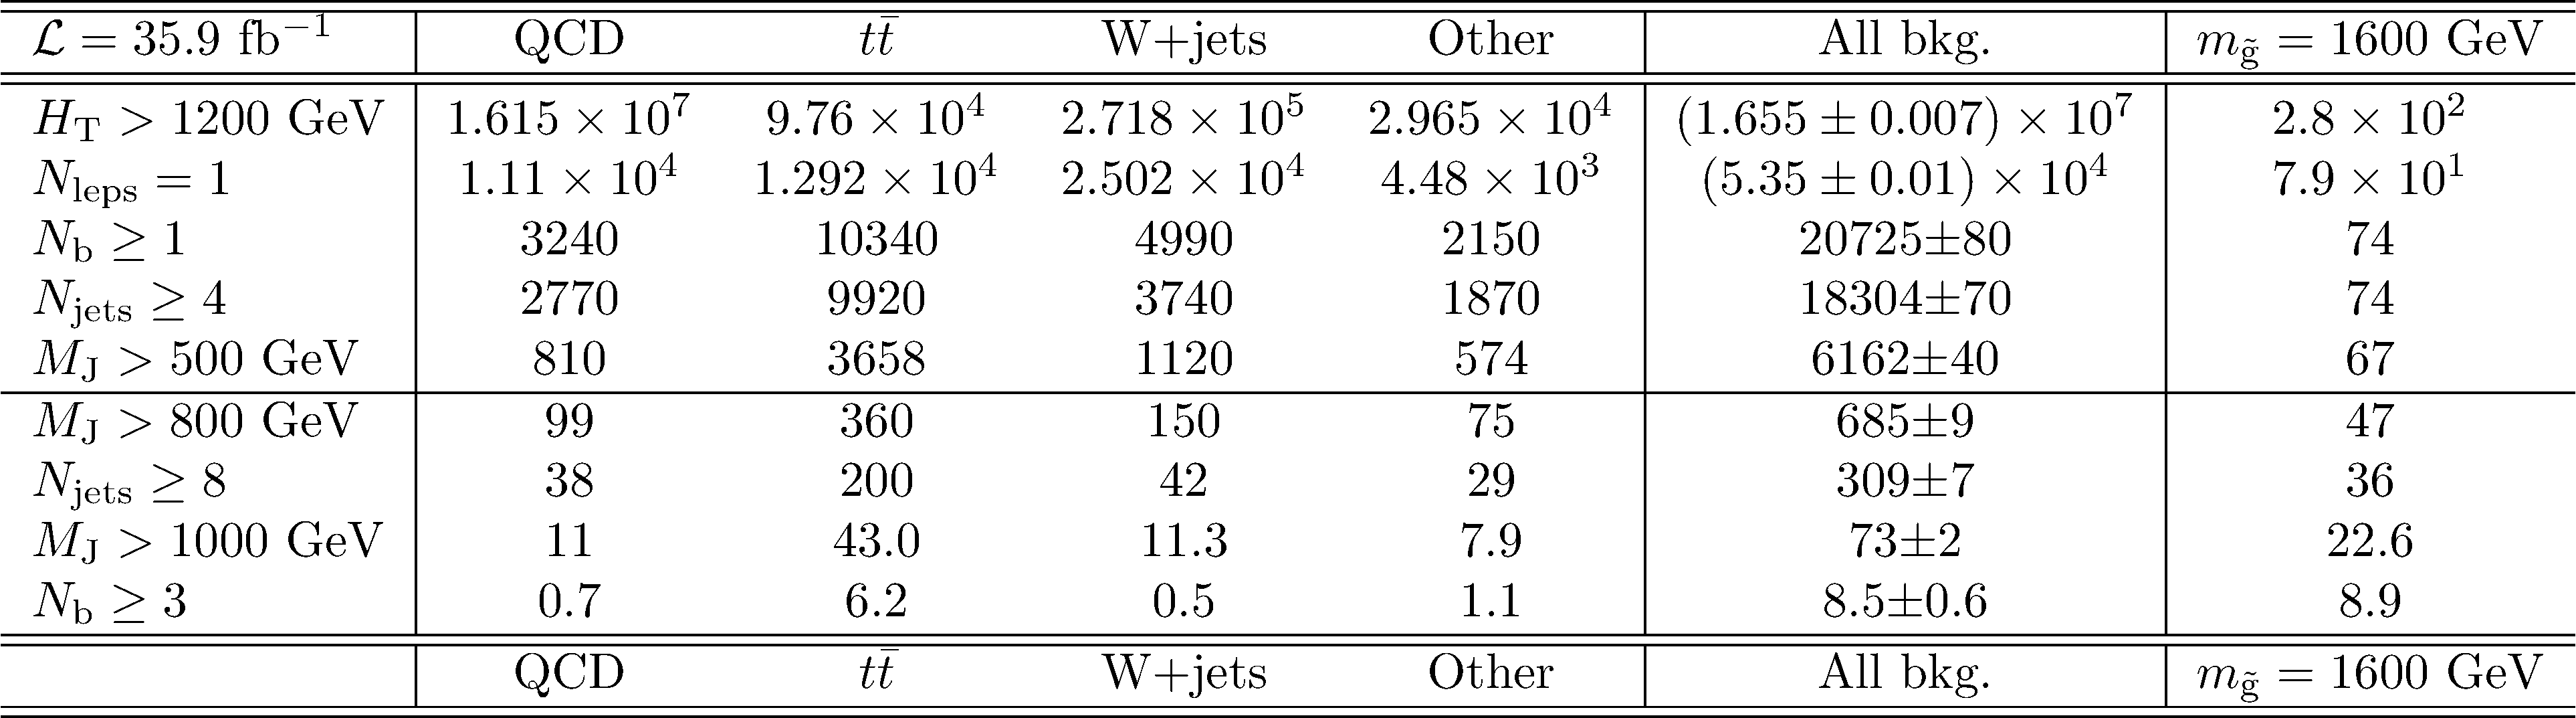
\includegraphics[angle=0,width=0.90\columnwidth]{fig/cutflow.pdf}
\caption{Expected yields in $35~\ifb$ from simulations of SM and signal processes.
Rows above the horizontal line correspond to requirements in the baseline selection, while those below correspond to additional kinematic cuts.}
\label{tab:cutflow}
\end{table}

The \baseHT cut sets the hadronic energy scale of the selected events and reduces contributions from processes other than QCD, \ttbar, and \Wjets.
At this point, the dominate background is QCD and is signicantly reduced by selecting events with \baseNleps, which leaves the QCD, \ttbar, and \Wjets contributions similar in scale.
In order to create a \ttbar dominant background, \baseNb is required as \ttbar events have at least two b-quark jets, while QCD and \Wjets contributions largely pass the selection by the mistagging of at least one jet.
Finally, the \baseNjets and \baseMJ cuts are applied in order to further increase the \ttbar purity of the analysis region.

A benefit of these selections is that the background is dominated by a single process, \ttbar, which reduces the complexity of the background prediction.
This is especially necessary as, after these cuts, the analysis region is on the kinematic tails of SM distributions where the physics is less well-modelled, typically requiring data-driven background predictions.

Lastly, the baseline selection requires that events pass a series of filters designed to remove poorly reconstructed events. 
These filters remove events with noise in the HCAL or ECAL, beam halo effects, jets that fail to pass quality criteria, and events with zero good PVs.

A final note of interest is that there is no requirement on the \MET, making this analysis sensitive to BSM models other than MFV SUSY that produce either little or no \MET in an event.
While the T1tbs model is used as a benchmark for interpreting results, to take advantage of this feature, this search is structured to be generically sensitive to high-mass signatures with large jet and bottom quark jet multiplicities, which are potential features of other BSM models.

\end{section}

\begin{section}{Trigger Efficiency}
The data sample used in this analysis is obtained by selecting events that pass a loose HLT selection.
In order to avoid biasing the selected sample, the HLT requirements must be loose enough that the selection efficiency is as high as possible and independent of any kinematic properties.
In particular, events must pass an \texttt{OR} of the \trigHT trigger, which requires an online-\HT of at least 900~\GeV and the \trigJet trigger, which at least one jet with online-\pT above 450~\GeV.

Figure~\ref{fig:ht_trigger} shows the performance of the \trigHT trigger as a function of \HT during the first 27.3~\ifb (Runs B-G, top-left), last 8.7~\ifb (Run H, top-right), and full dataset (Runs B-H, bottom).
The trigger performances are measured in a data sample collected using the \trigEle trigger and offline requirements of at least one electron and at least 4 jets.
While the trigger efficiency for Runs B-G is 100\% after the trigger plateau of roughly $\HT = 1000~\GeV$, the trigger efficiency only performs with 80\% efficiency in Run H.
This inefficiency was caused by an issue with an updated trigger implementation that erroneously excluded high \pT jets from the online-\HT calculation.
This effect corresponds to an overall trigger efficiency of 95\%, corresponding to a loss of about 2~\ifb of data.

\begin{figure}[tbp!]
\centering
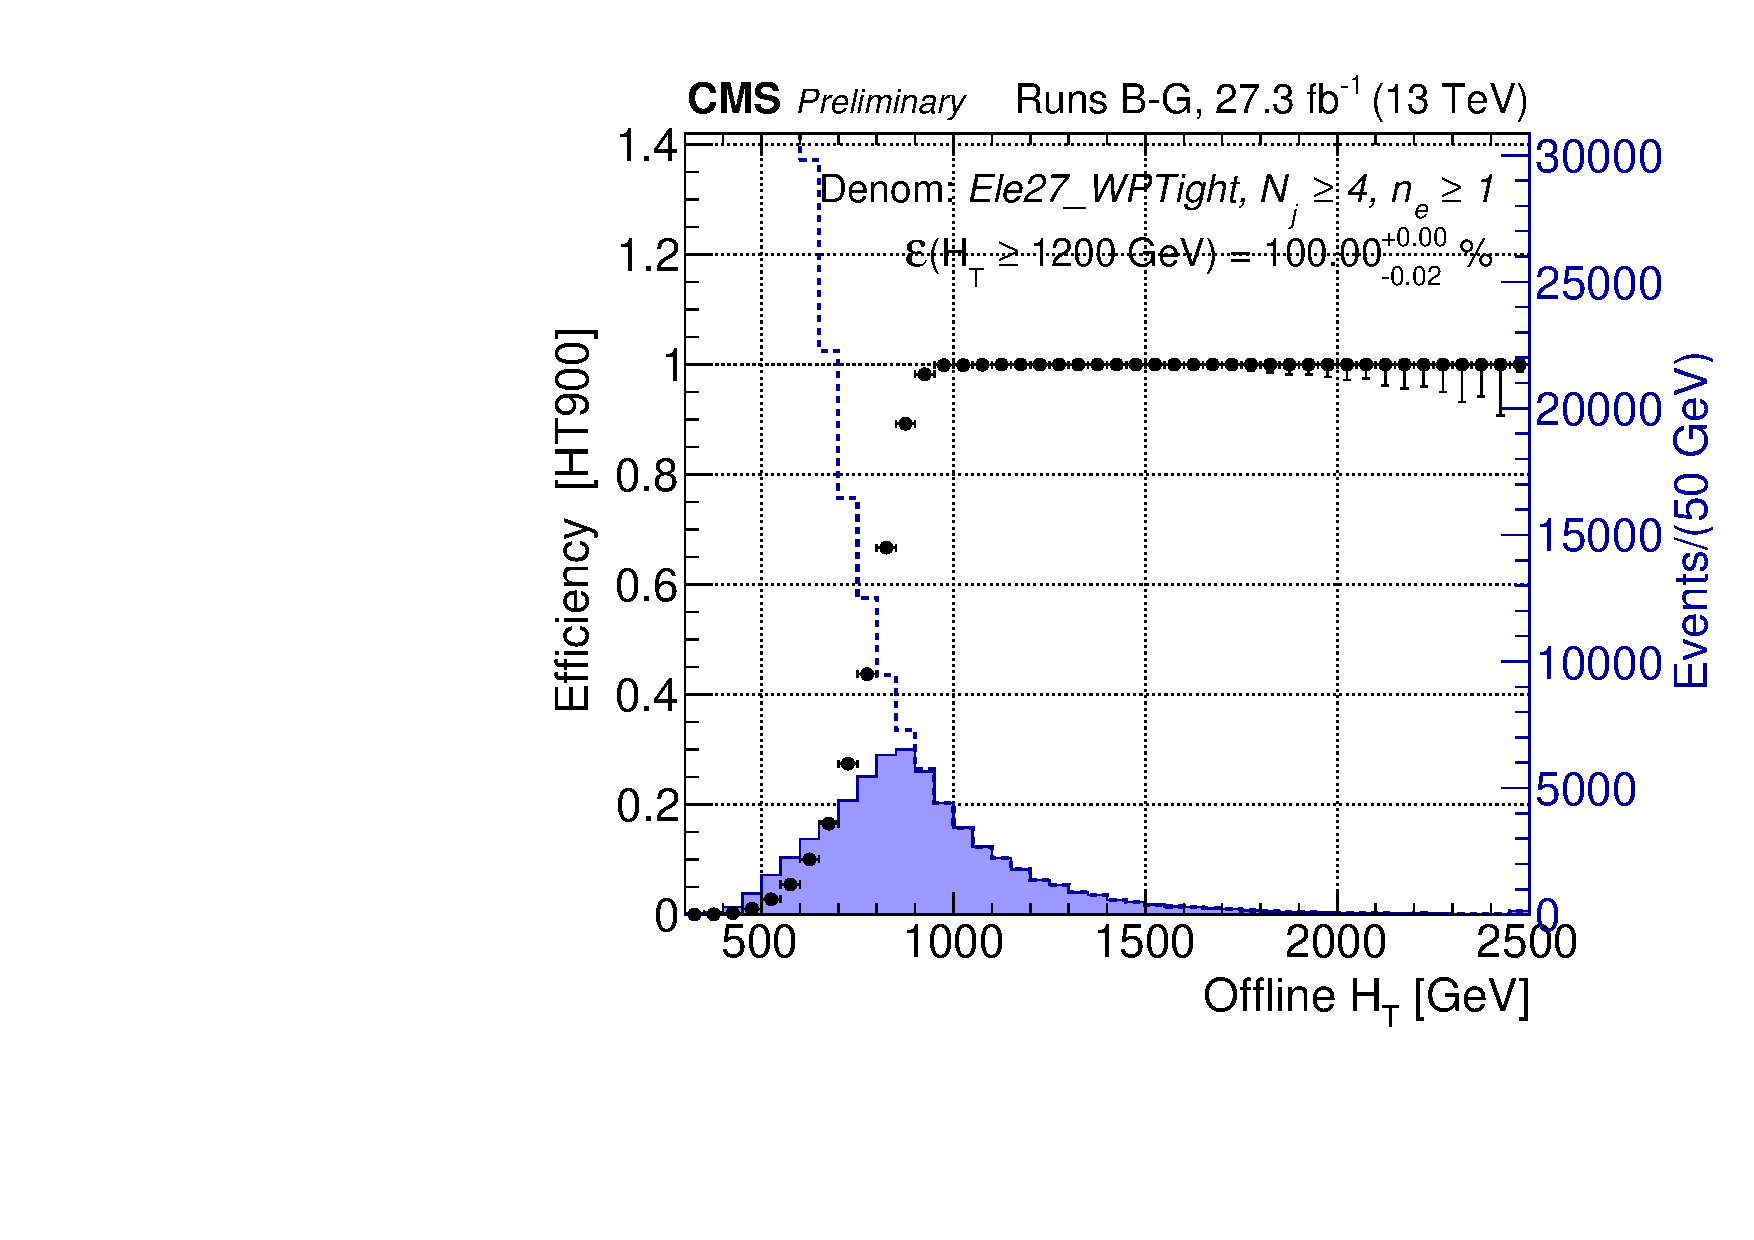
\includegraphics[angle=0,width=0.45\columnwidth]{fig/trig_ht_runsbg.pdf}
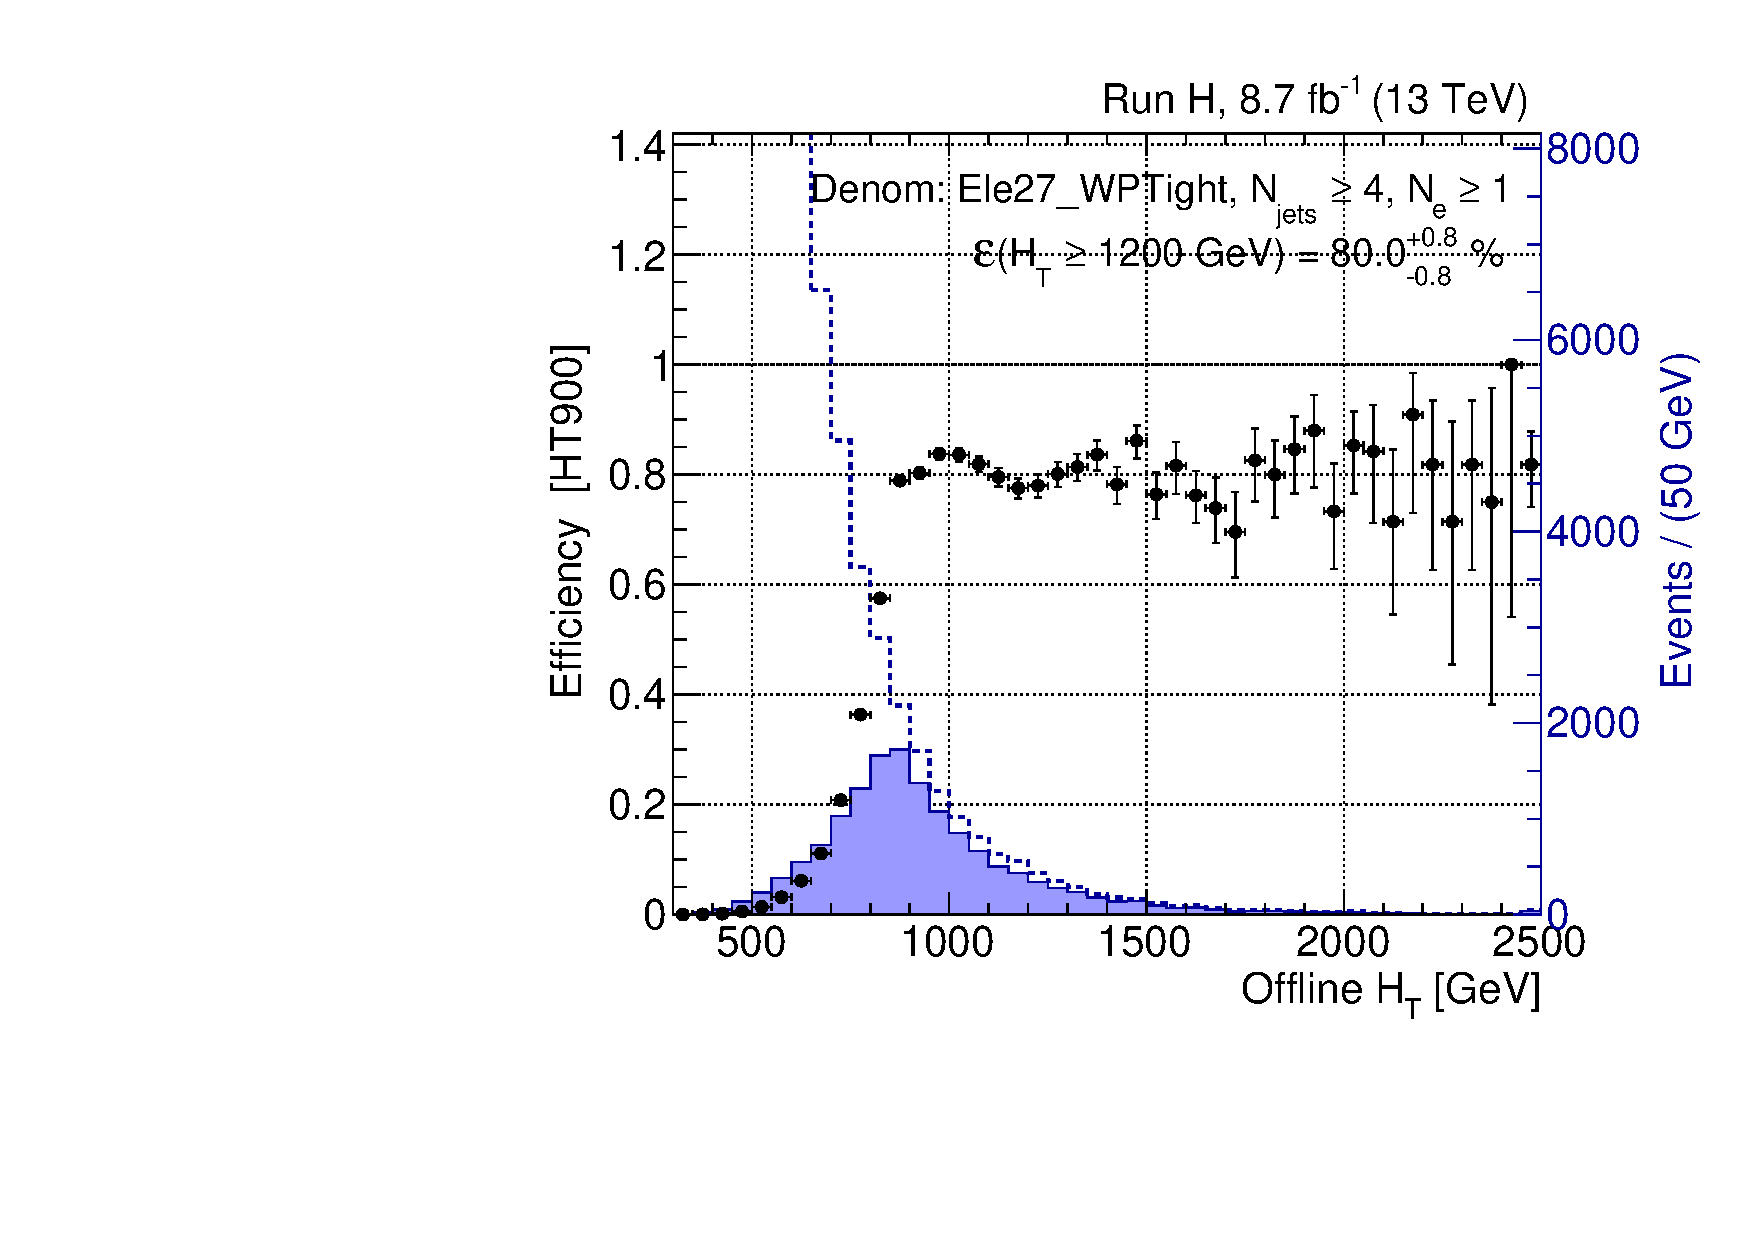
\includegraphics[angle=0,width=0.45\columnwidth]{fig/trig_ht_runh.pdf}
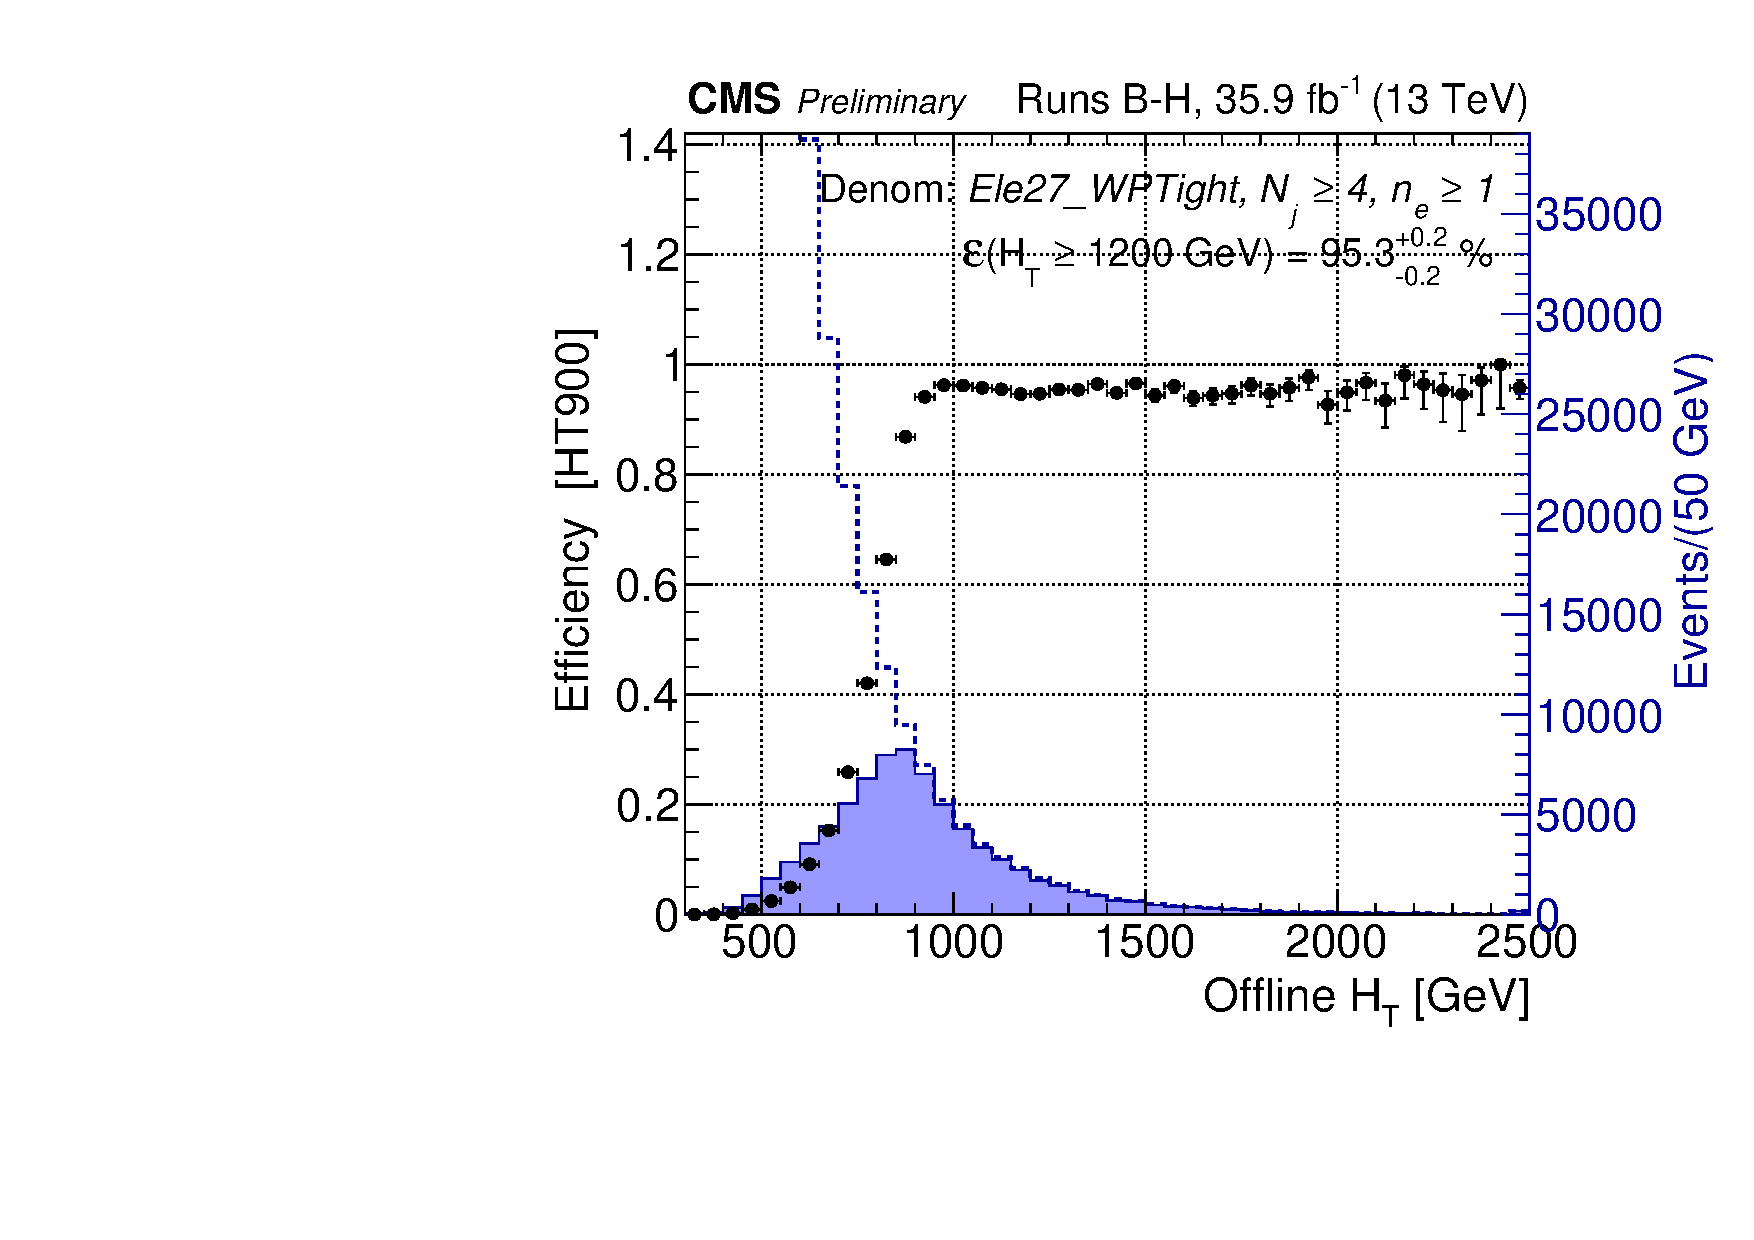
\includegraphics[angle=0,width=0.45\columnwidth]{fig/trig_ht_runsbh.pdf}
\caption{Trigger efficiency for \trigHT as a function of \HT in Runs B-G (top-left), Run H (top-right), and full dataset (bottom). 
The efficiences are measured using a data sample collected with the \trigEle trigger and an offline requiement of at least one electron and at least four jets.}
\label{fig:ht_trigger}
\end{figure}

In order to recover this inefficiency, events passing the \trigJet trigger are included in the collected data sample.
To pass this trigger, events must have at least one very high \pT jets, i.e. $\gtrsim 450~\GeV$, which provides complementary efficiency where the \trigHT trigger is inefficient.
Figure~\ref{fig:ht_jet_trigger} shows the performance as a function of \HT of the \trigJet trigger in Runs B-H (top-left) and the combination of the \trigHT and \trigJet in Run H (middle) and in the full dataset (bottom), measured with a dataset collected with \trigEle and offline requirements of at least one electron and at least 4 jets.
The inclusion of the \trigJet trigger restores the overall trigger efficiency to essentially 100\% in both Run H and the entire dataset.

\begin{figure}[tbp!]
\centering
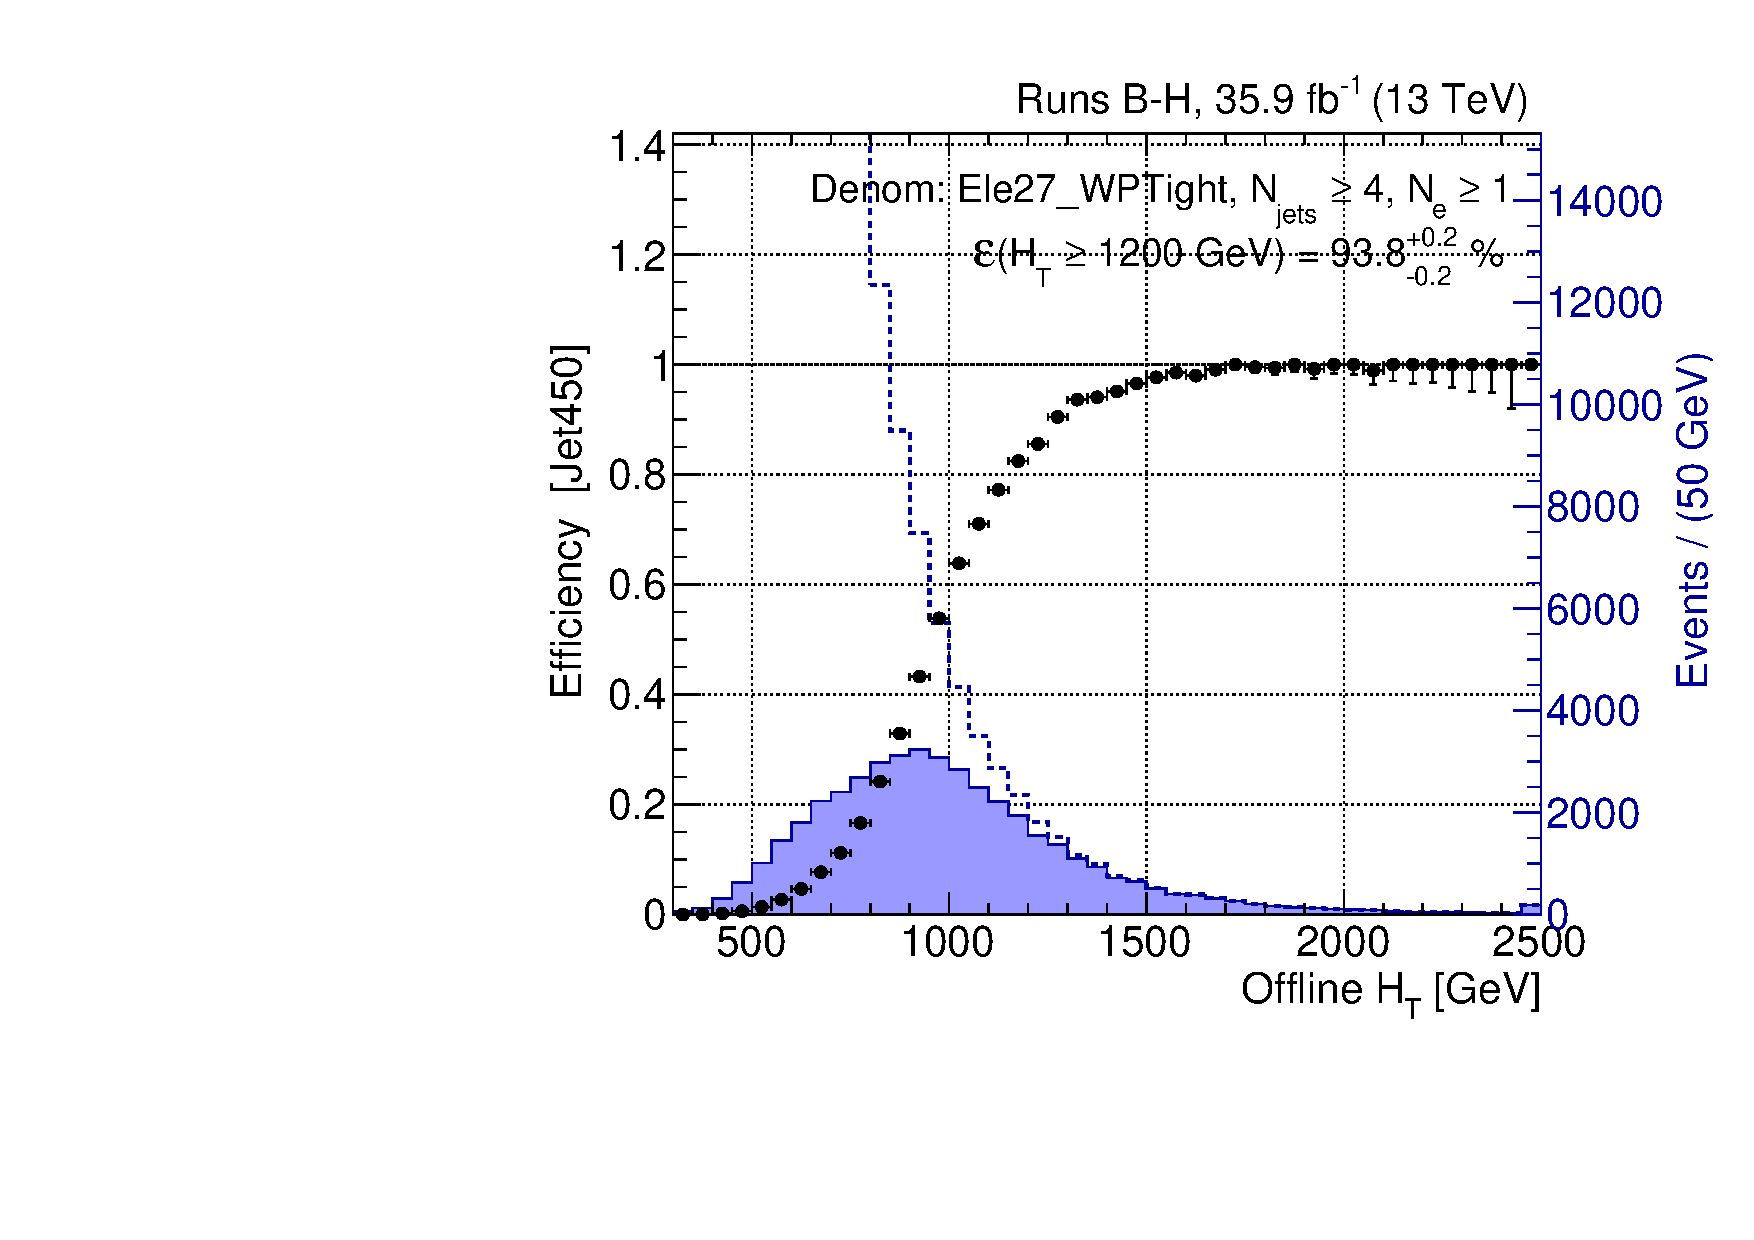
\includegraphics[angle=0,width=0.45\columnwidth]{fig/trig_jet_runsbh.pdf}
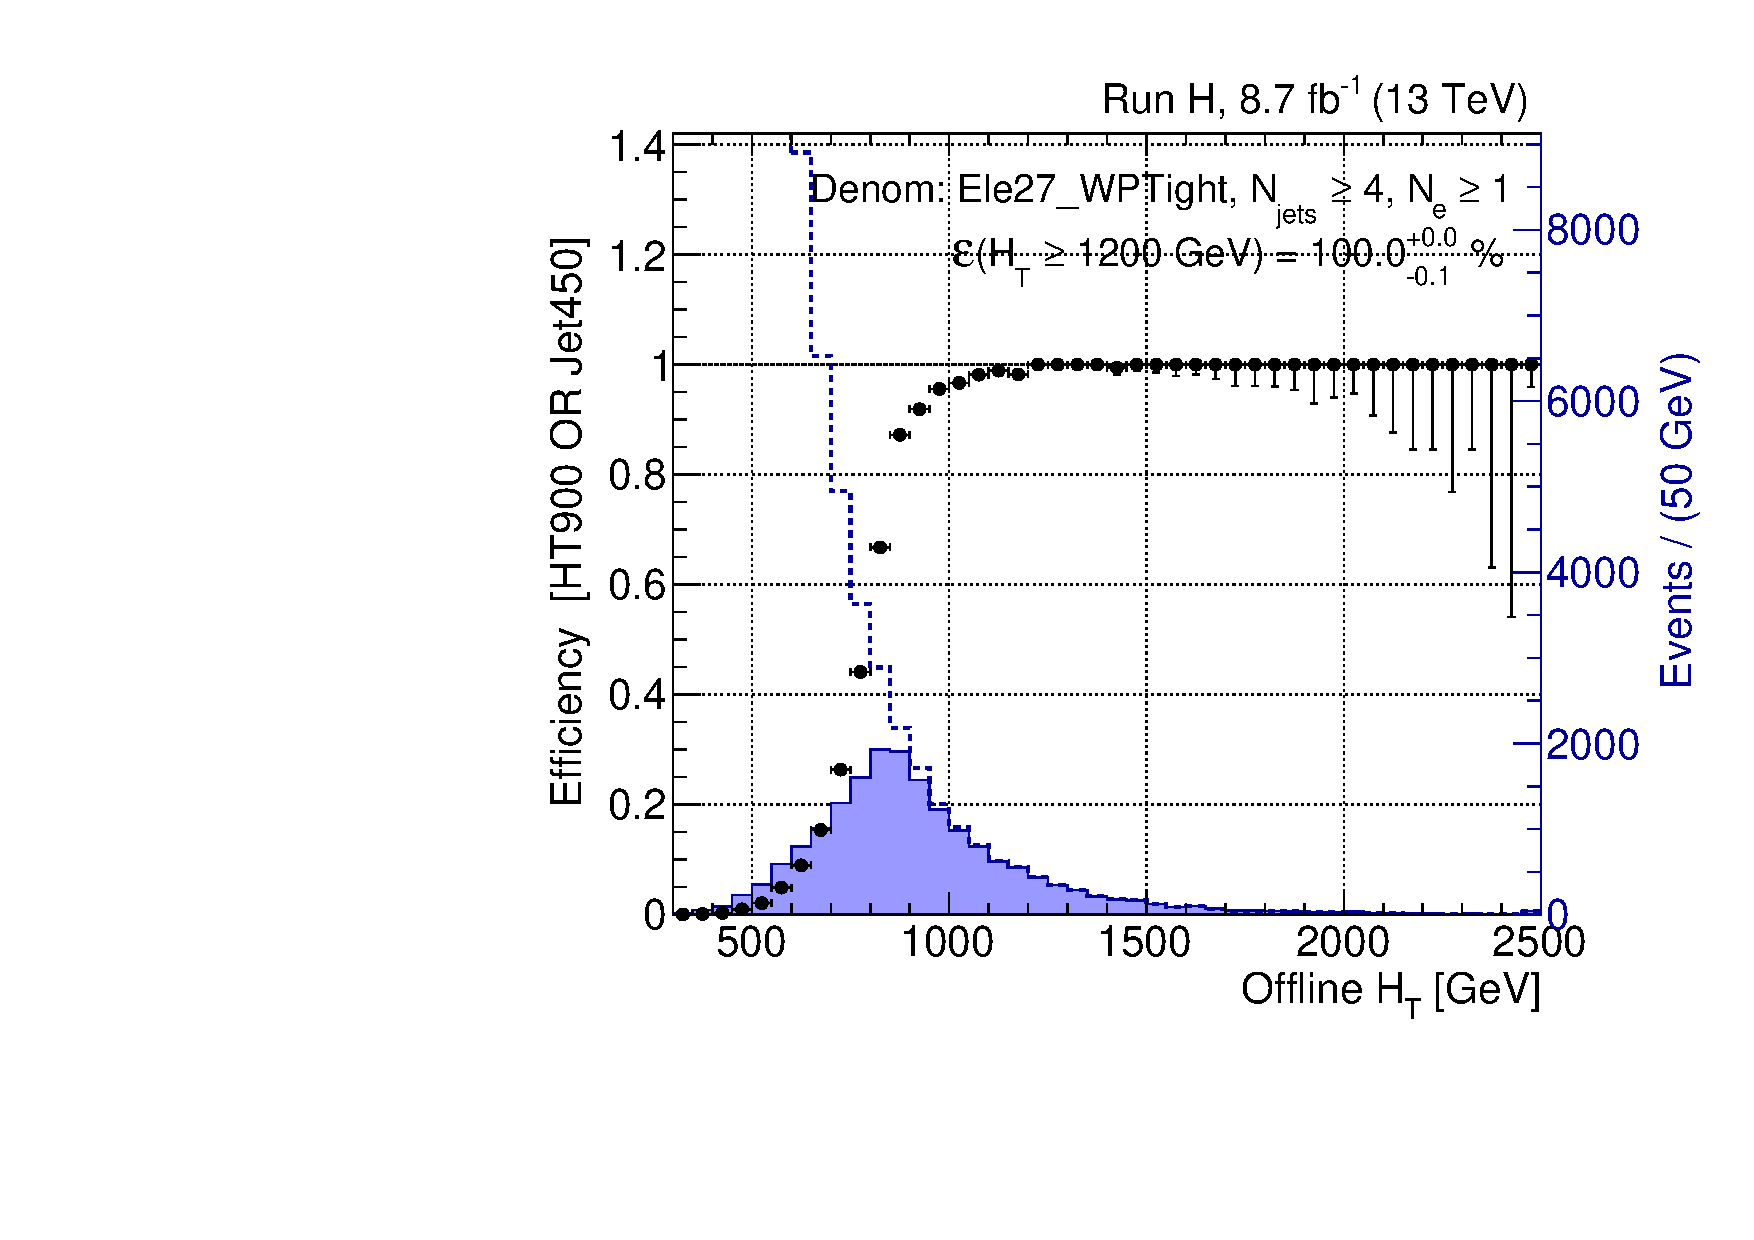
\includegraphics[angle=0,width=0.45\columnwidth]{fig/trig_ht_jet_runh.pdf}
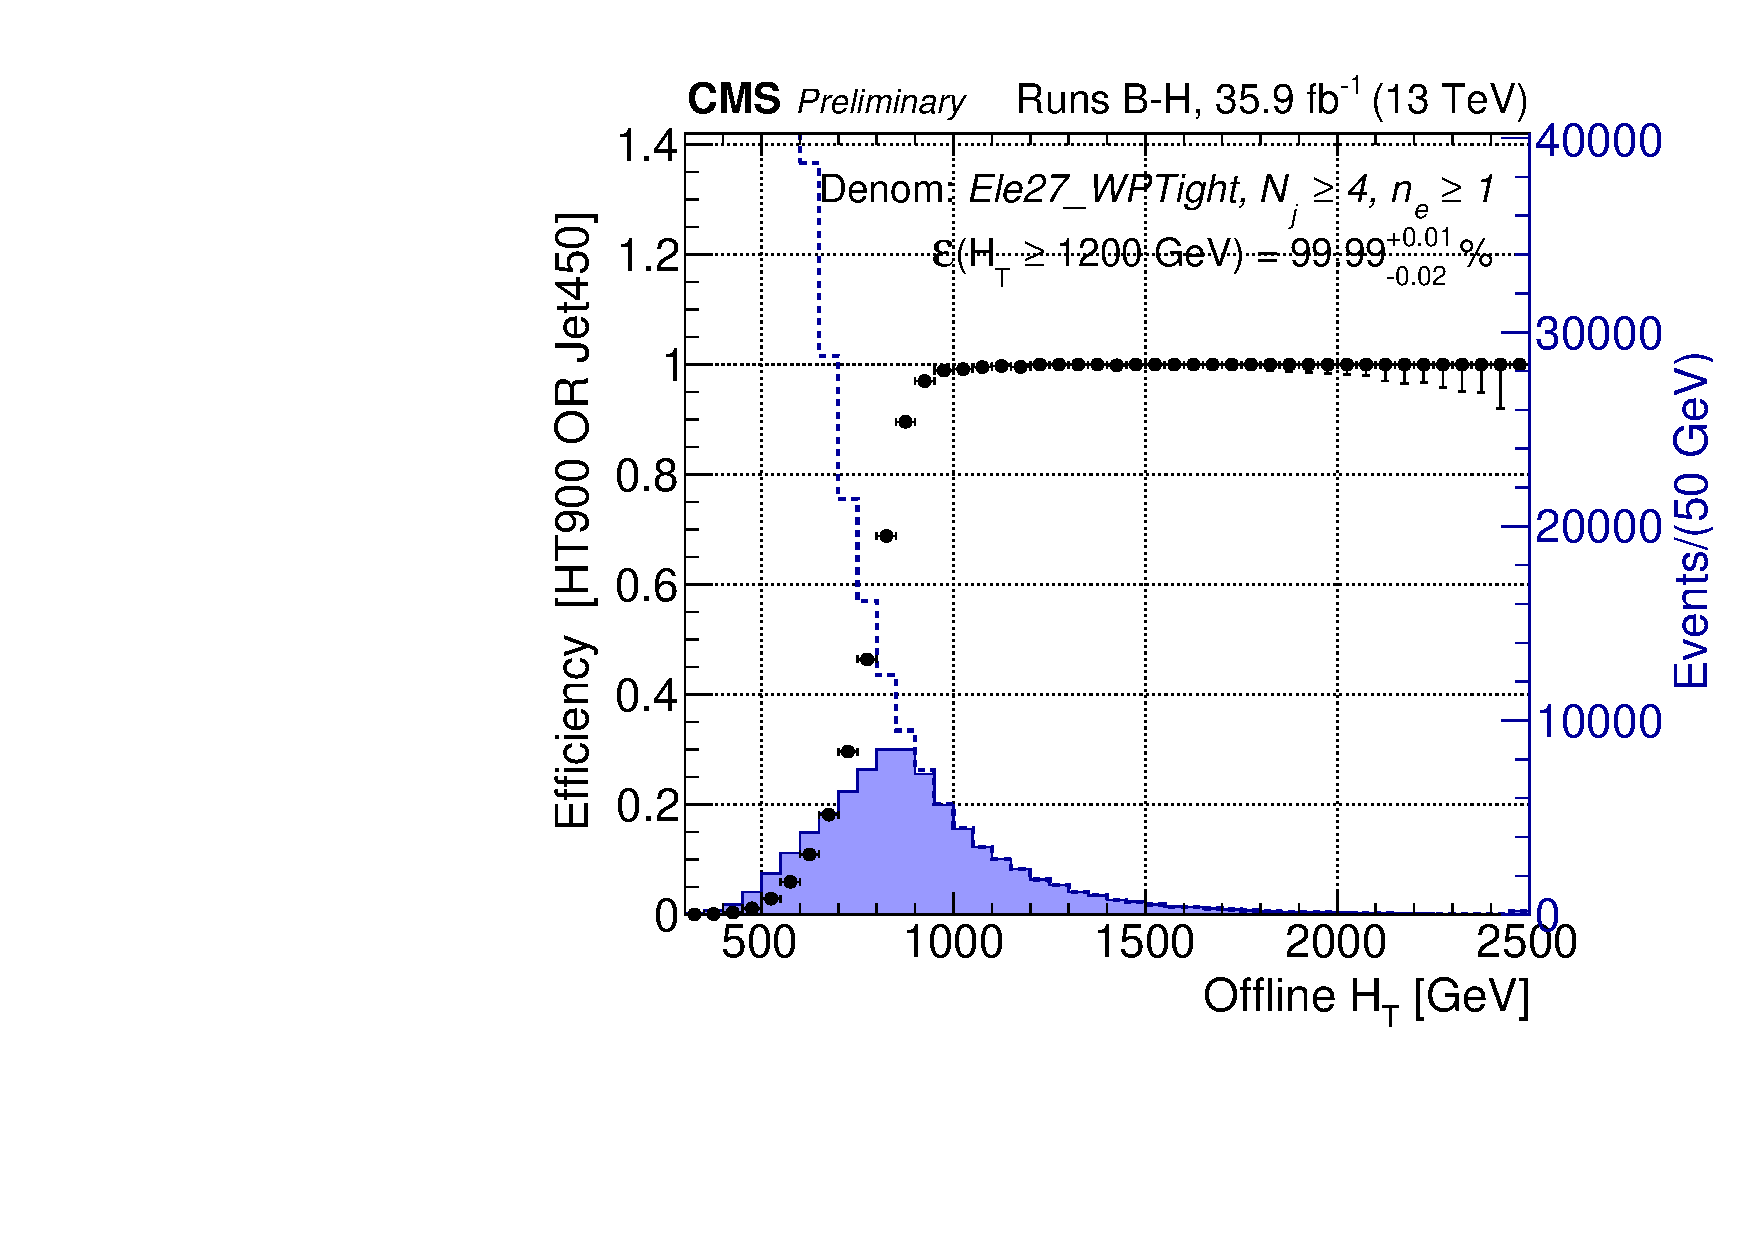
\includegraphics[angle=0,width=0.45\columnwidth]{fig/trig_ht_jet_runsbh.pdf}
\caption{Trigger efficiency as a function of \HT for \trigJet in the full dataset (top-left) and for the combination of \trigHT and \trigJet in Run H (top-right) and the full dataset (bottom).
The efficiences are measured using a data sample collected with the \trigEle trigger and an offline requiement of at least one electron and at least four jets.}
\label{fig:ht_jet_trigger}
\end{figure}

This trigger efficiency, however, does not necessarilly correspond to the efficiency for signal events.
A lower bound on the signal efficiency can be estimated by considering that the \trigJet trigger is fully efficient for jets with $\pT > 500~\GeV$ and 80\%-95\% of simulated signal events (depending on the mass of the gluino) have a jet with $pT > 500~\GeV$.
Thus, in the worst case scenario, the addition of the \trigJet trigger is still expected to recover at least 85\% of the lost signal efficiency in Run H.
This results in an efficiency of at least 97\% in Run H and over 99\% for the full dataset for signal events.

Lastly, to ensure that there is no kinematic bias in the trigger efficiency either inherently or residually from effects of the online-\HT calculation issue, the trigger efficency is measured as a function of \MJ, \Njets, and \Nb.
The measurements, shown in Figure~\ref{fig:kinvars_trigger} are done in a data sample collected with the \trigEle trigger and an offline requirement of at least one electron, at least four jets, and \baseHT.
The resulting efficiencies are all consistent with 100\% and no kinematic bias is observed.

\begin{figure}[tbp!]
\centering
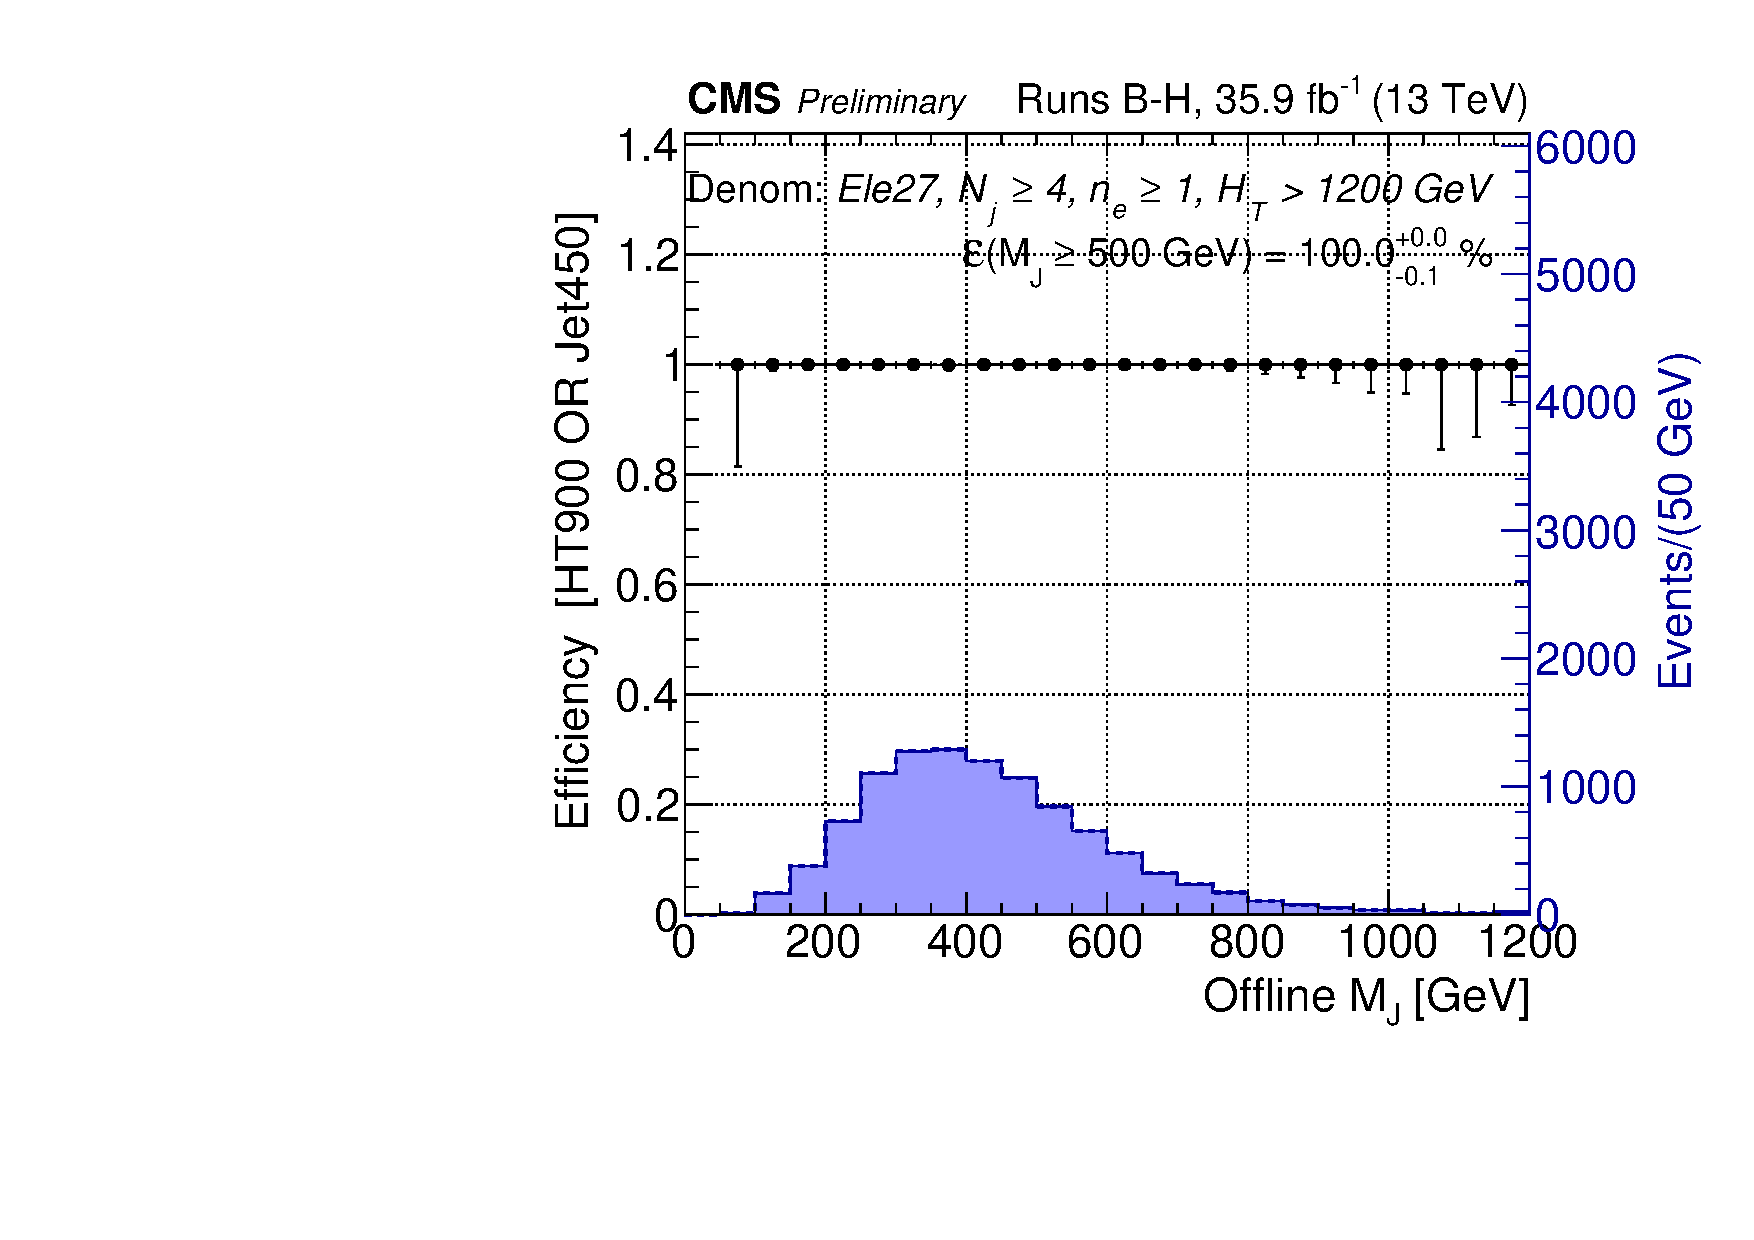
\includegraphics[angle=0,width=0.45\columnwidth]{fig/trig_ht_jet_mj_runsbh.pdf}
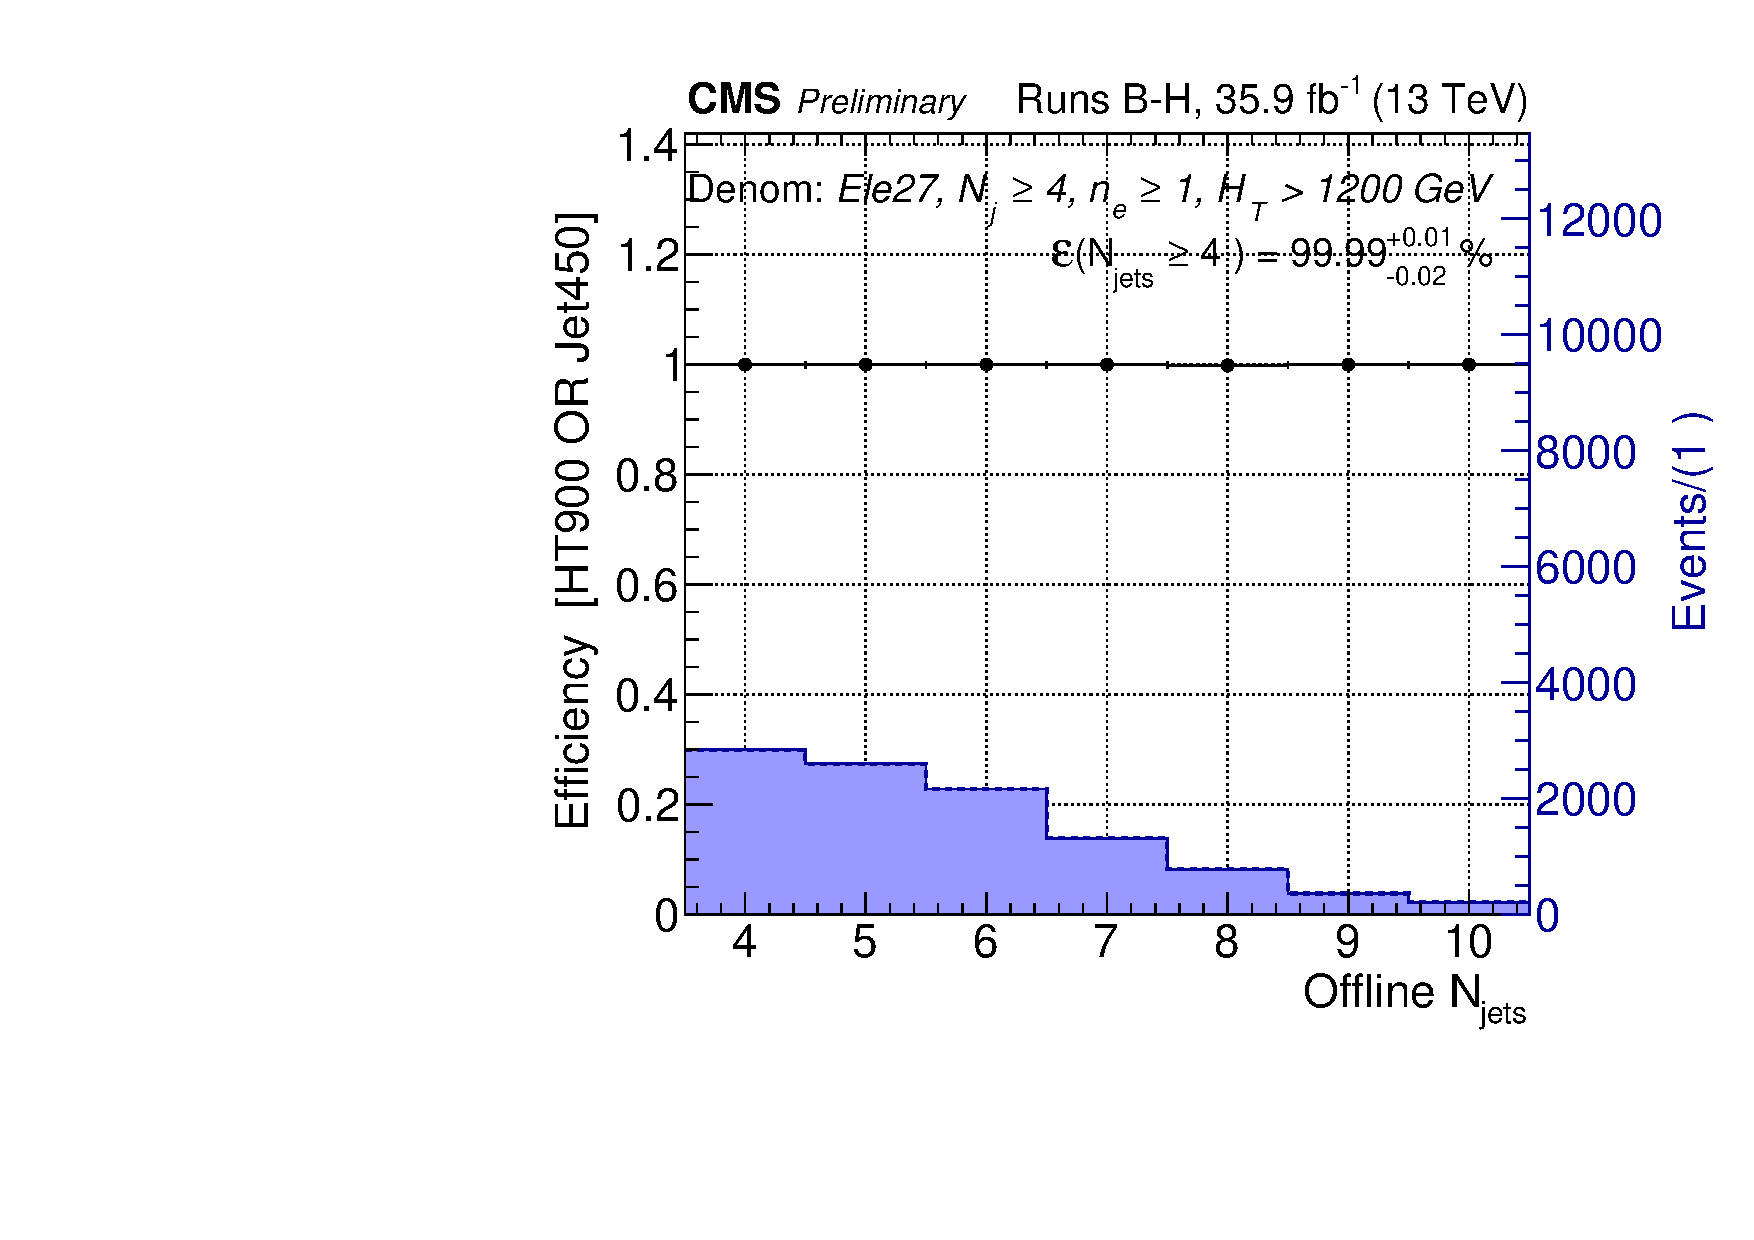
\includegraphics[angle=0,width=0.45\columnwidth]{fig/trig_ht_jet_njets_runsbh.pdf}
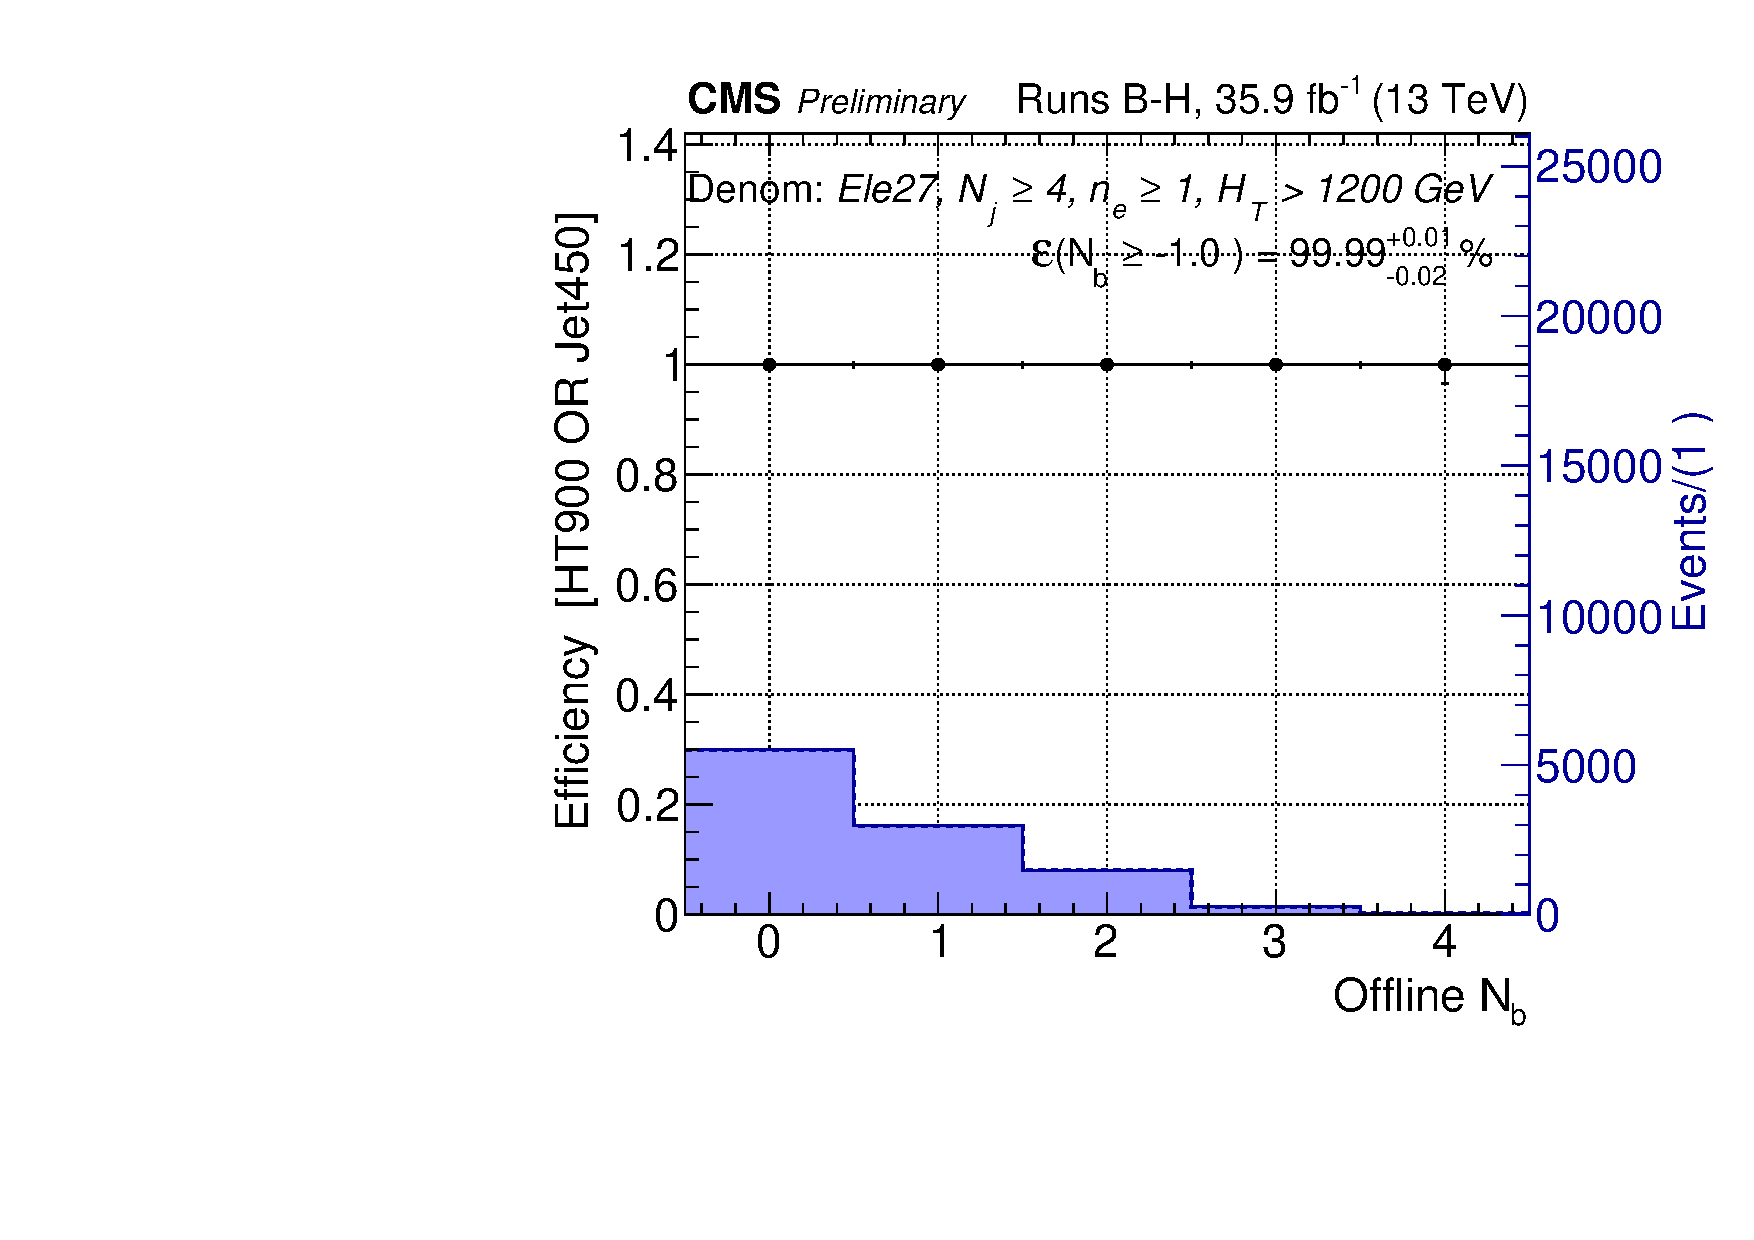
\includegraphics[angle=0,width=0.45\columnwidth]{fig/trig_ht_jet_nb_runsbh.pdf}
\caption{Trigger efficiency as a function of \MJ (top-left), \Njets (top-right), and \Nb (bottom) for the combination of the \trigHT and \trigJet triggers in the full dataset.
The efficiencies are measured using a data sample collected using the \trigEle trigger and an offline requirement of at least one electron, at least four jets, and \baseHT.}
\label{fig:kinvars_trigger}
\end{figure}

\end{section}

\begin{section}{Analysis Binning}
After the baseline selection, the background is dominated by \ttbar events with small contributions from \Wjets and QCD production.
There are additional rare background processes, jointly noted as ``Other'', with tiny, but non-zero contributions that arise from single top quark, \ttW, \ttZ, \ttH, \tttt, and Drell-Yan production.

In order to further increase the signal-to-background ratio, as well as create background-dominated control regions, the analysis region is binned with respect to \Njets and \MJ. 
The \Njets bins are defined as $4 \leq \Njets \leq 5$, $6 \leq \Njets \leq 7$, and $\Njets \geq 8$.
Each \Njets bin is further split into bins of $500 < \MJ \leq 800~\GeV$, $800 < \MJ \leq 1000~\GeV$, and $\MJ > 1000~\GeV$, with the exception of the $4 \leq \Njets \leq 5$ bin for which the two highest \MJ bins are combined due to the limited data sample size in the $\MJ \geq 1000~\GeV$ bin.
A diagram representing this binning is shown in Figure~\ref{fig:analysis_regions}.
The low-\Njets, low-\MJ bins are expected to be background-dominated and are used as control regions for constraining sytematics and for validating the prediction methodology, while the high-\Njets, high-\MJ bins are used as signal regions.

\begin{figure}[tbp!]
\centering
\begin{tabular}{ |c|c|c|c| }
\hline
\multirow{2}{*}{\MJ [\GeV]}          &  \multicolumn{3}{c|}{\Njets}                      \\ \cline{2-4}
                                     &  4--5                        & 6--7  &  $\geq 8$  \\ \hline
500--800                             &  CR                          & CR    &  SR        \\ \hline
800--1000                            &  \multirow{2}{*}{CR}         & SR    &  SR        \\ \cline{1-1} \cline{3-4}
$> 1000$                             &                              & SR    &  SR        \\ \hline
\end{tabular}
\caption{Illustration depicting the \Njets, \MJ binning after the baseline selection, with control and signal region bins denoted by ``CR'' and ``SR'', respectively.}
\label{fig:analysis_regions} 
\end{figure}

Within each \Njets and \MJ bin, the \Nb distribution is examined for evidence of new physics and is separated into bins of $\Nb = 1$, 2, 3, and $\geq 4$.
The two lowest \Nb bins are used to provide constraints on the background normalizations and systematic uncertainites, while the higher \Nb bins are the most sensitive to potential signals due to its larger signal-to-background ratios.

In total, this analysis has 8 kinematic regions--3 control and 5 signal regions with four \Nb bins per kinematic region.
The simulated \Nb distribution of the SM background processes and a signal model with $\mglu = 1600~\GeV$ for the control and signal regions 
are shown in Figure~\ref{fig:nb_cr_dists} and Figure~\ref{fig:nb_sr_dists}, respectively.

\begin{figure}[tbp!]
\centering
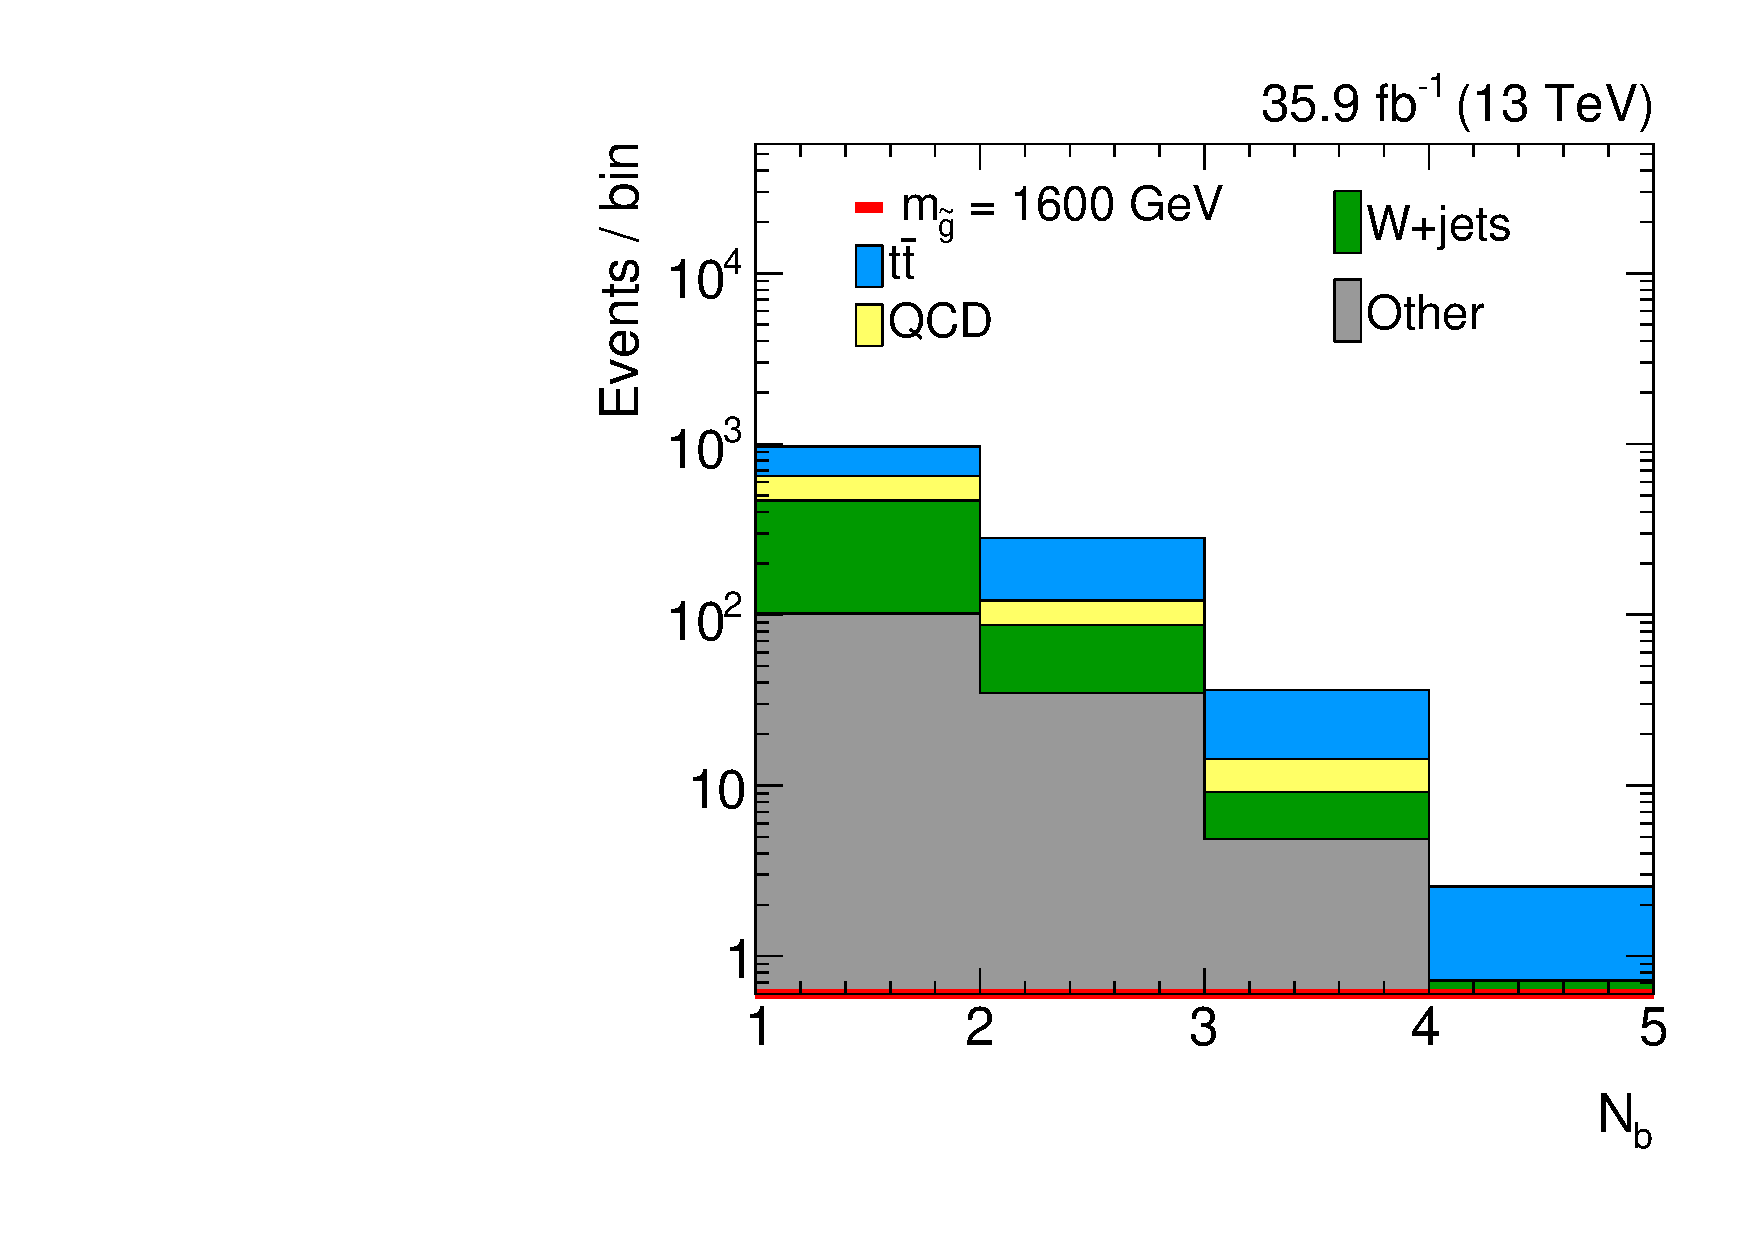
\includegraphics[angle=0,width=0.35\columnwidth]{fig/nb_nlep1_nj45_lowmj.pdf}
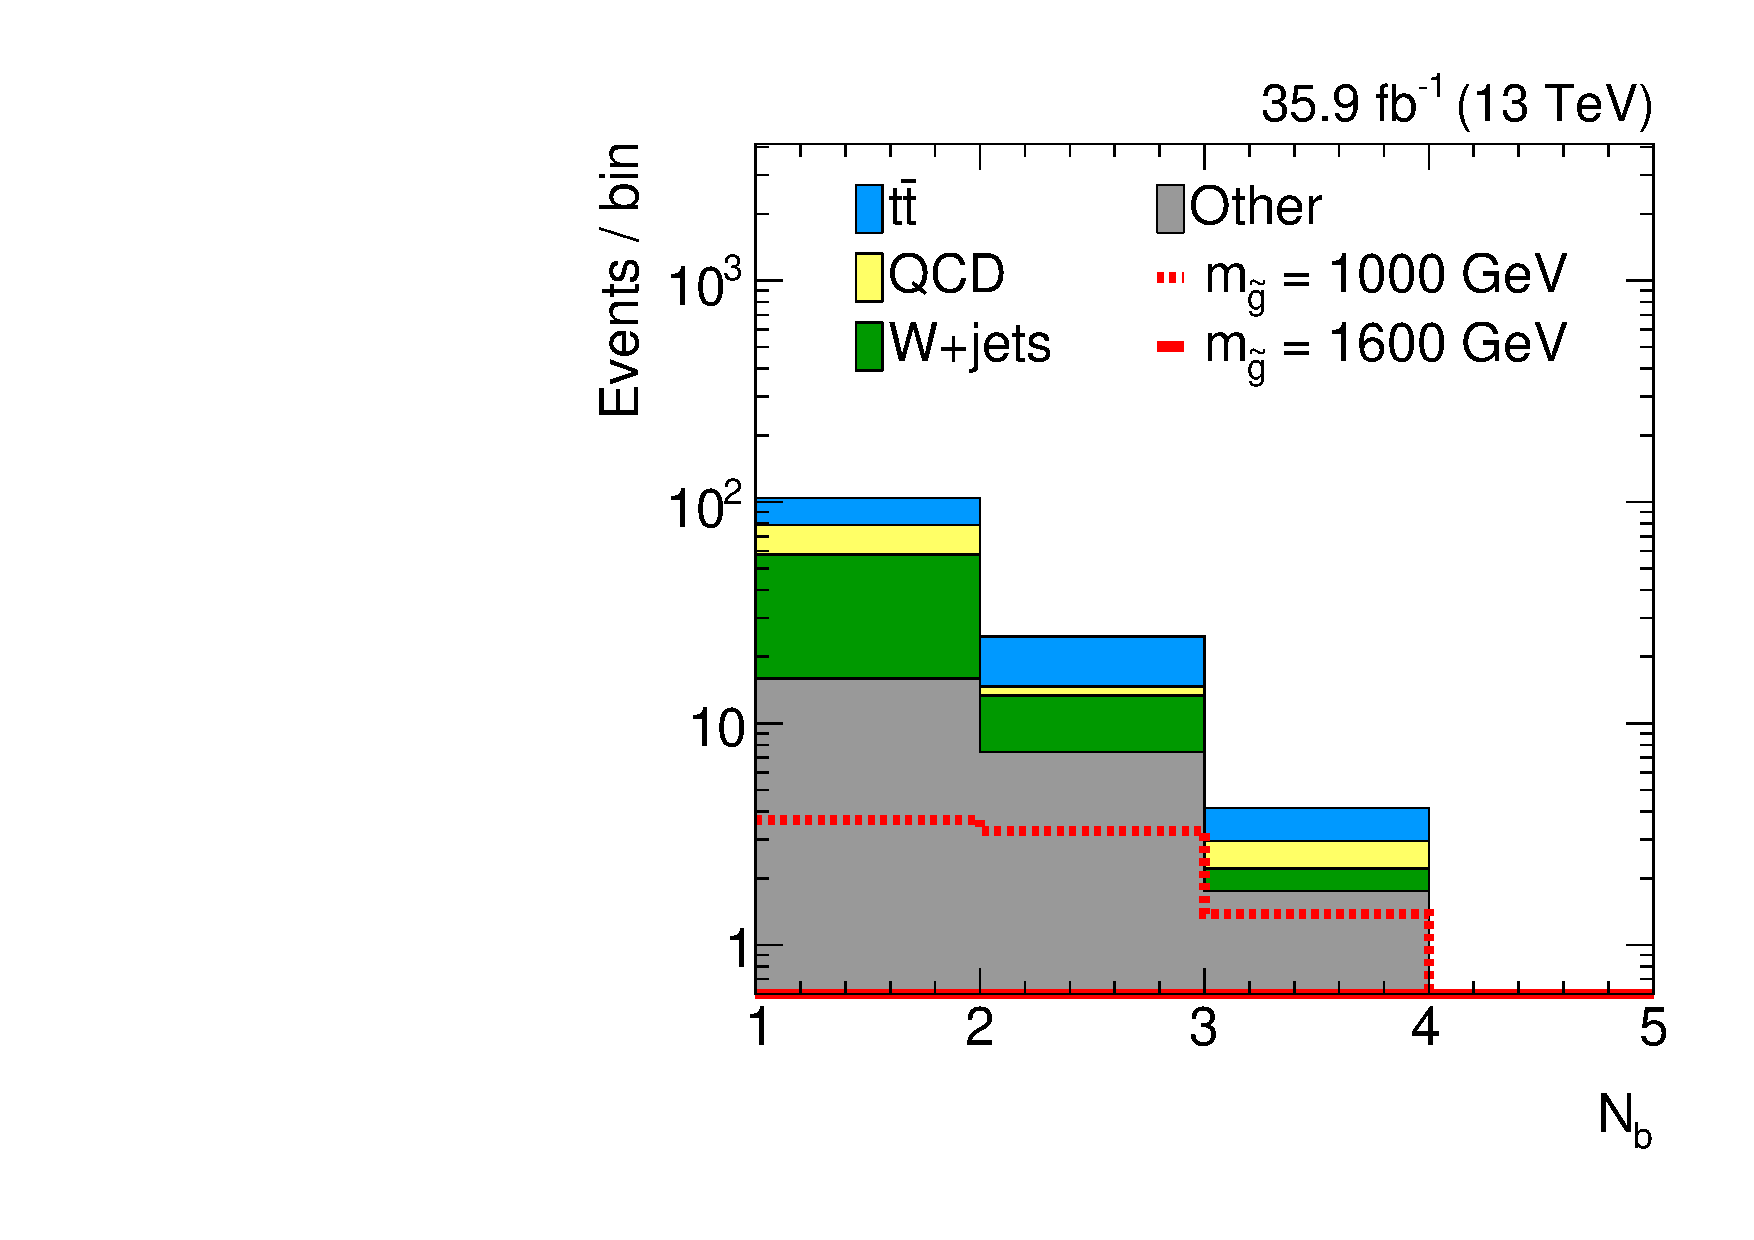
\includegraphics[angle=0,width=0.35\columnwidth]{fig/nb_nlep1_nj45_highmj.pdf}
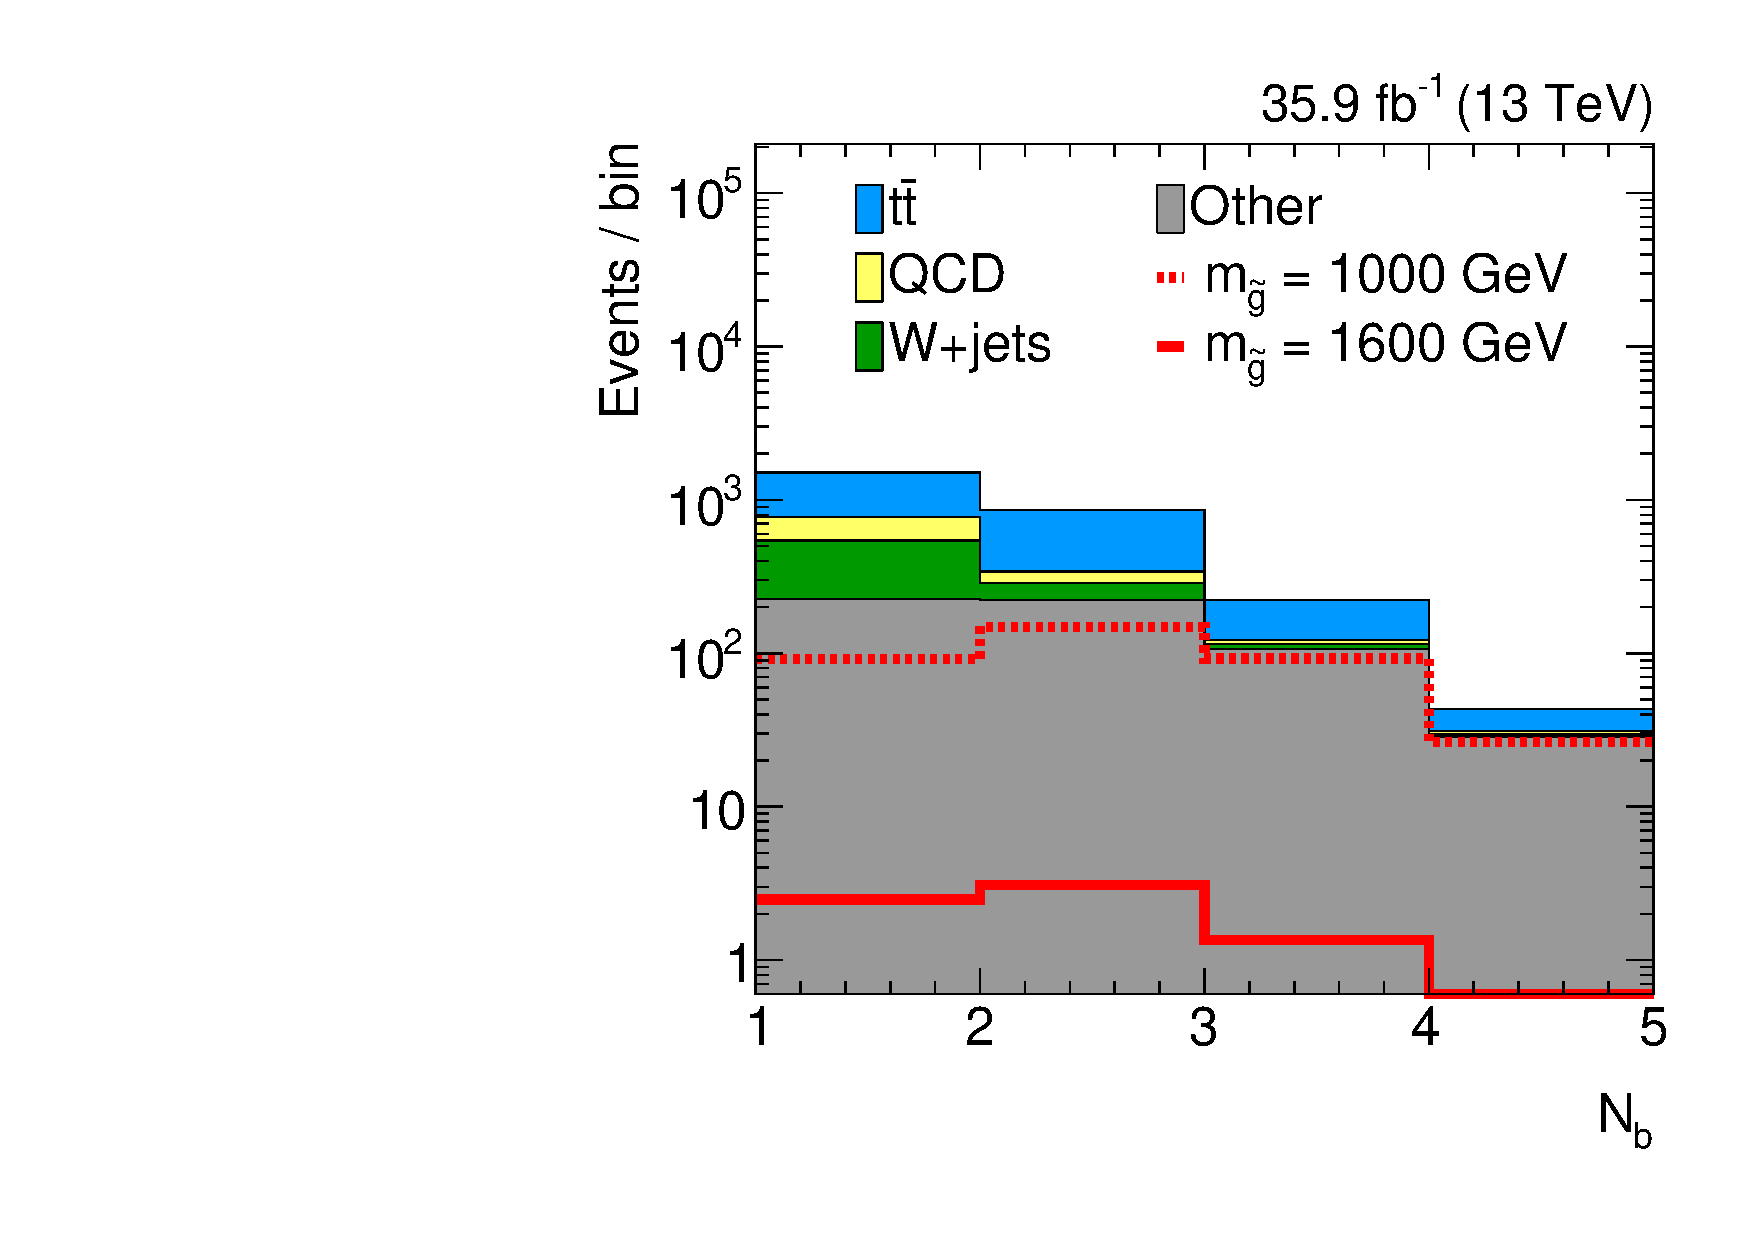
\includegraphics[angle=0,width=0.35\columnwidth]{fig/nb_nlep1_nj67_lowmj.pdf}
\caption{The simulated \Nb distribution for background and signal processes in the control region bins.
The top-left plot corresponds to the $4 \leq \Njets \leq 5$, $500 \leq \MJ \leq 800~\GeV$ bin, the top-right plot to the $5 \geq \Njets \geq 6$, $\MJ \geq 800~\GeV$ bin, and the bottom plot to the $6 \leq \Njets \leq 7$, $500 \leq \MJ \leq 800~\GeV$ bin.}
\label{fig:nb_cr_dists}
\end{figure}

\begin{figure}[tbp!]
\centering
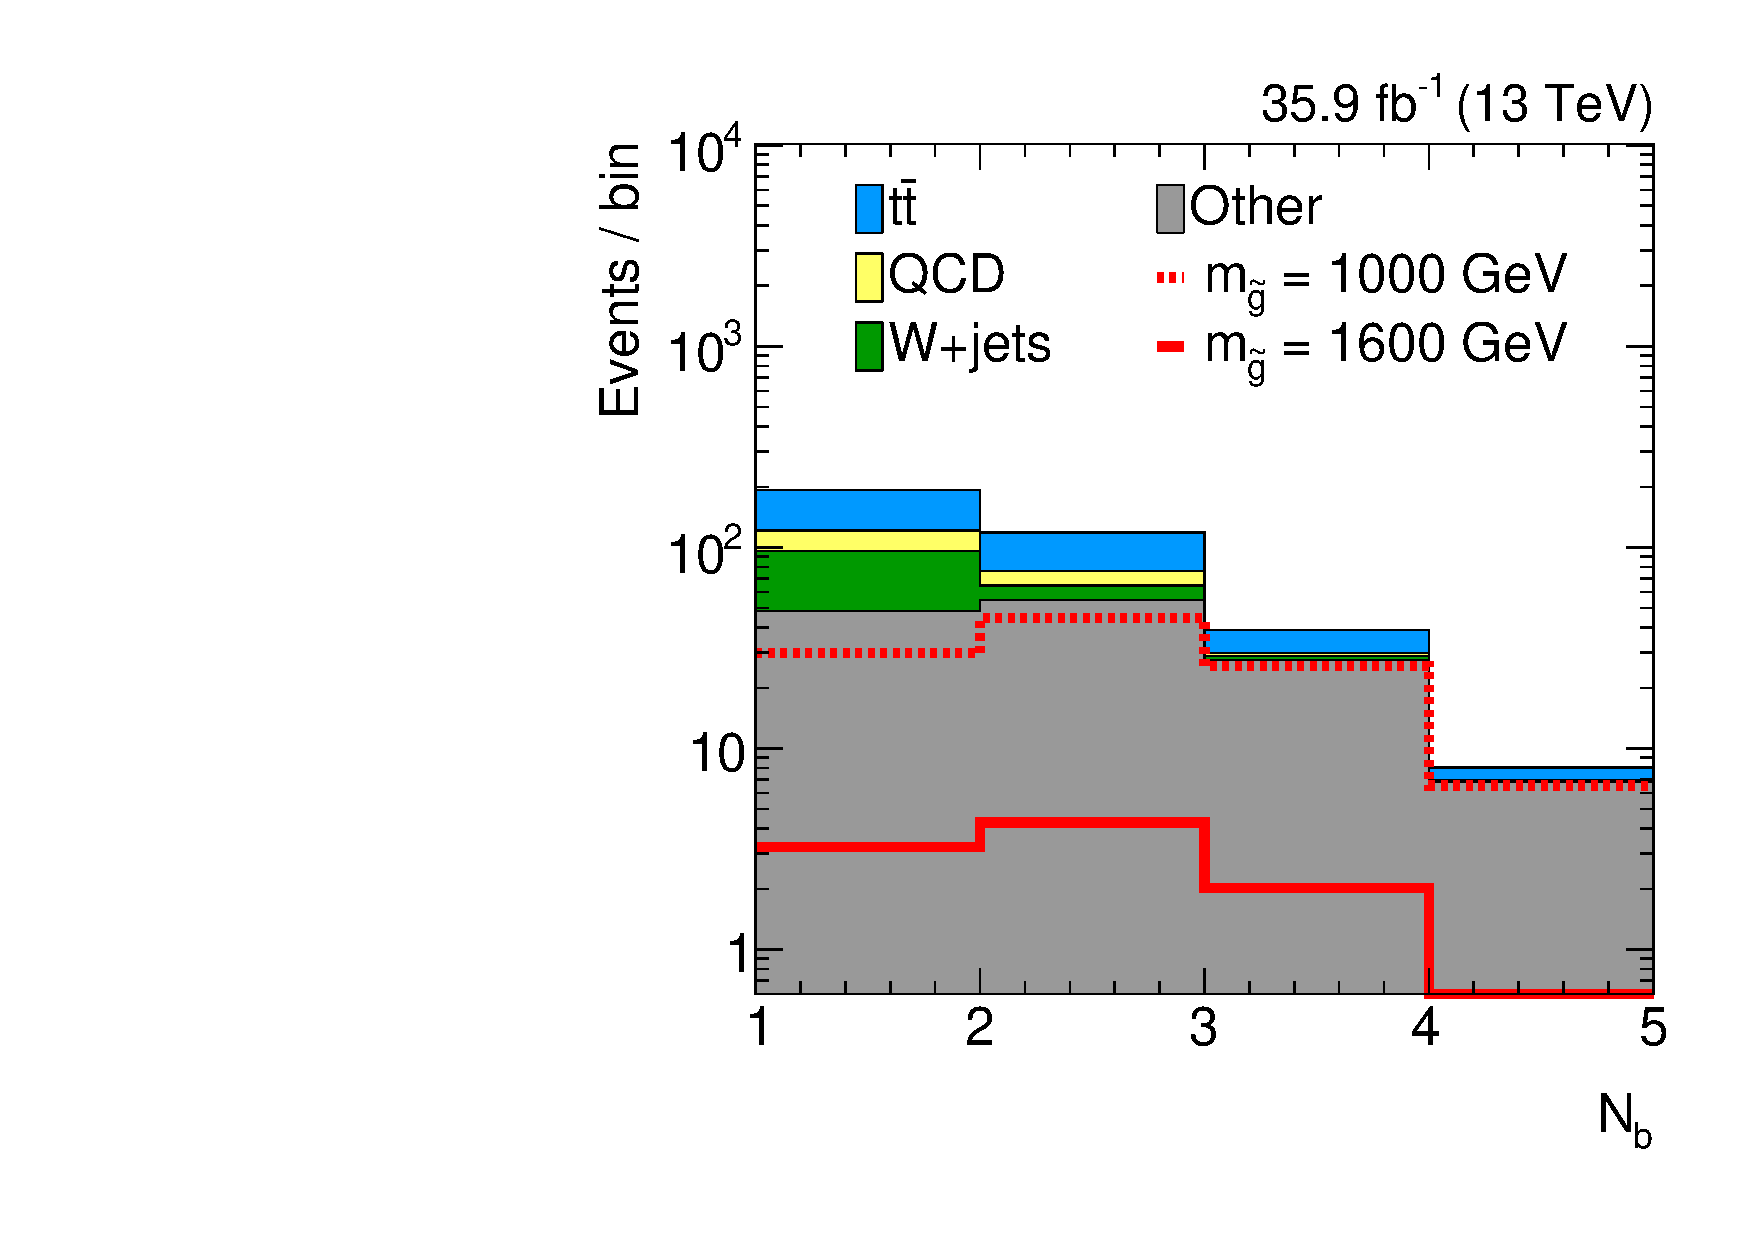
\includegraphics[angle=0,width=0.35\columnwidth]{fig/nb_nlep1_nj67_highmj.pdf}
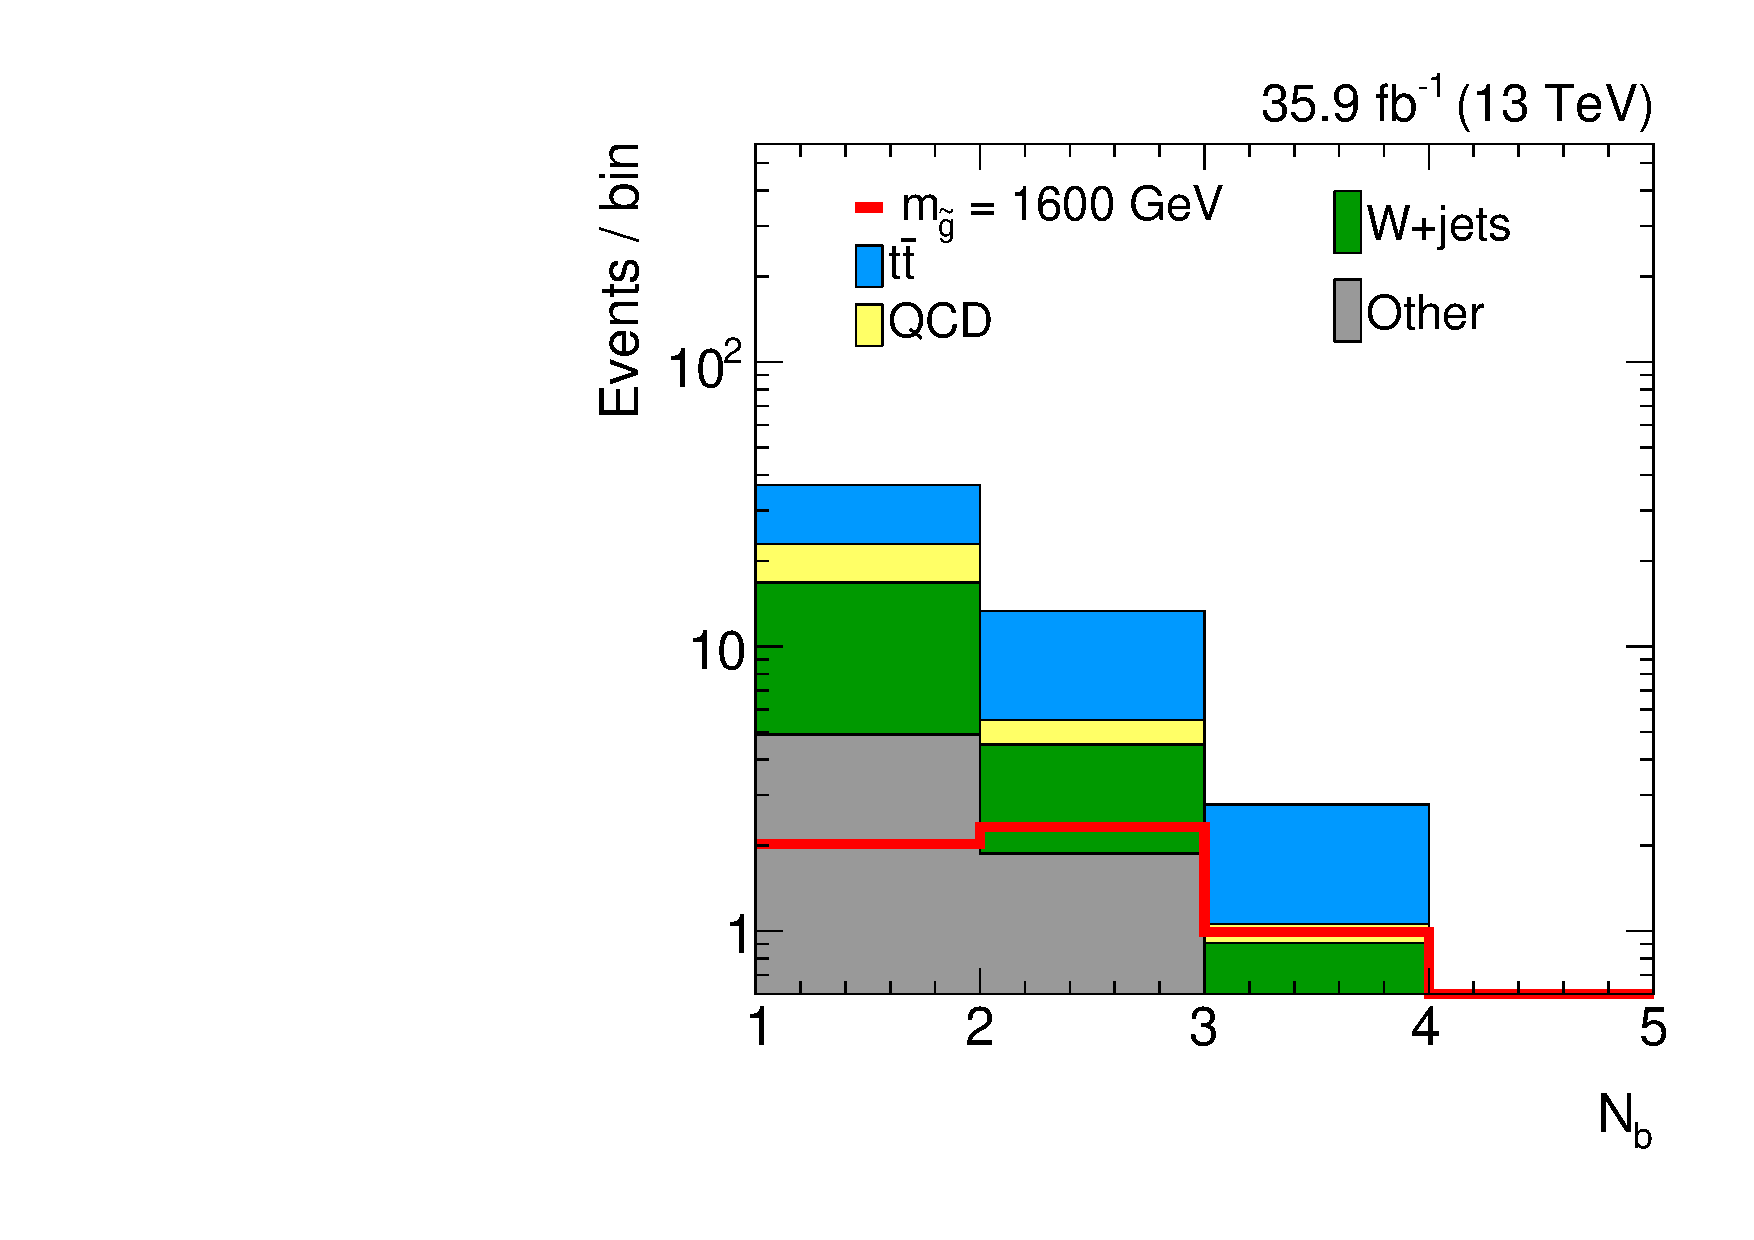
\includegraphics[angle=0,width=0.35\columnwidth]{fig/nb_nlep1_nj67_vhighmj.pdf}
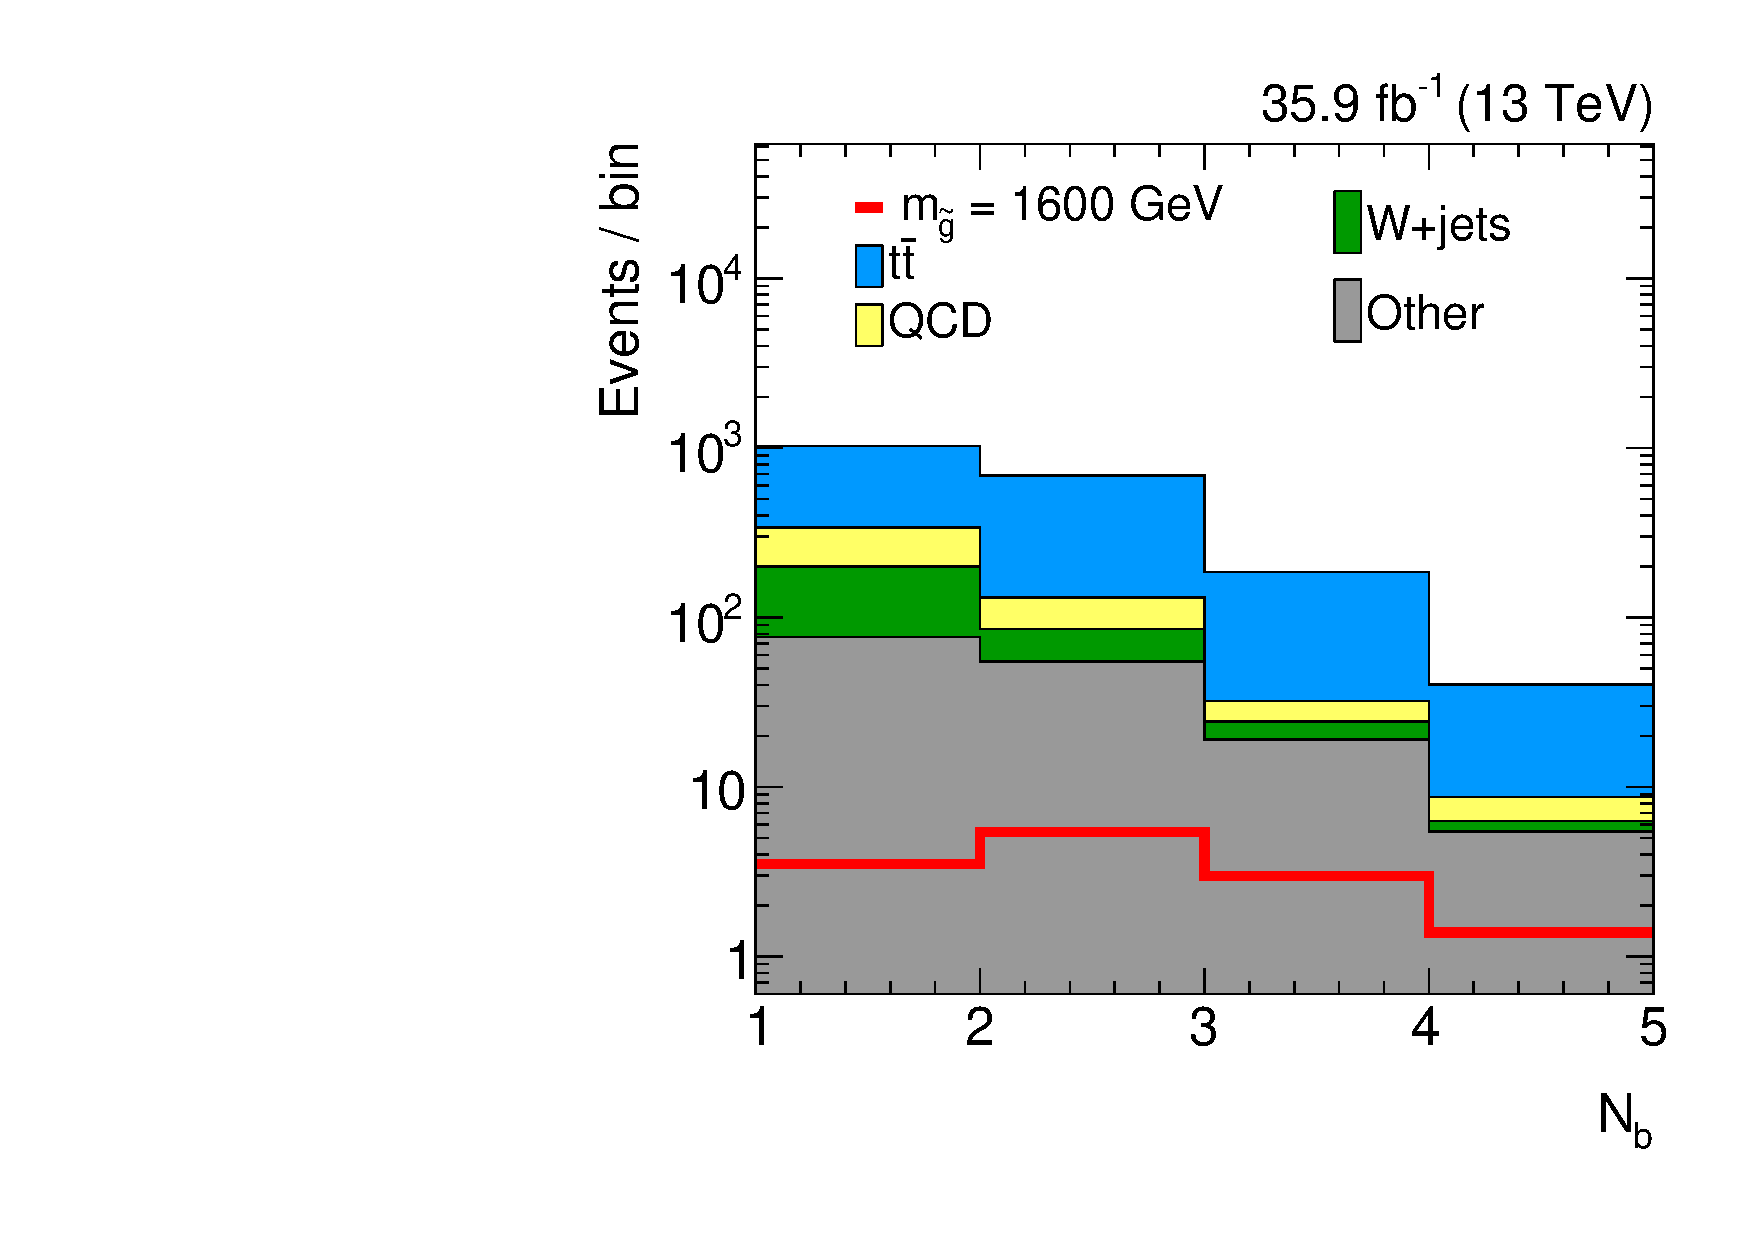
\includegraphics[angle=0,width=0.35\columnwidth]{fig/nb_nlep1_nj8_lowmj.pdf}
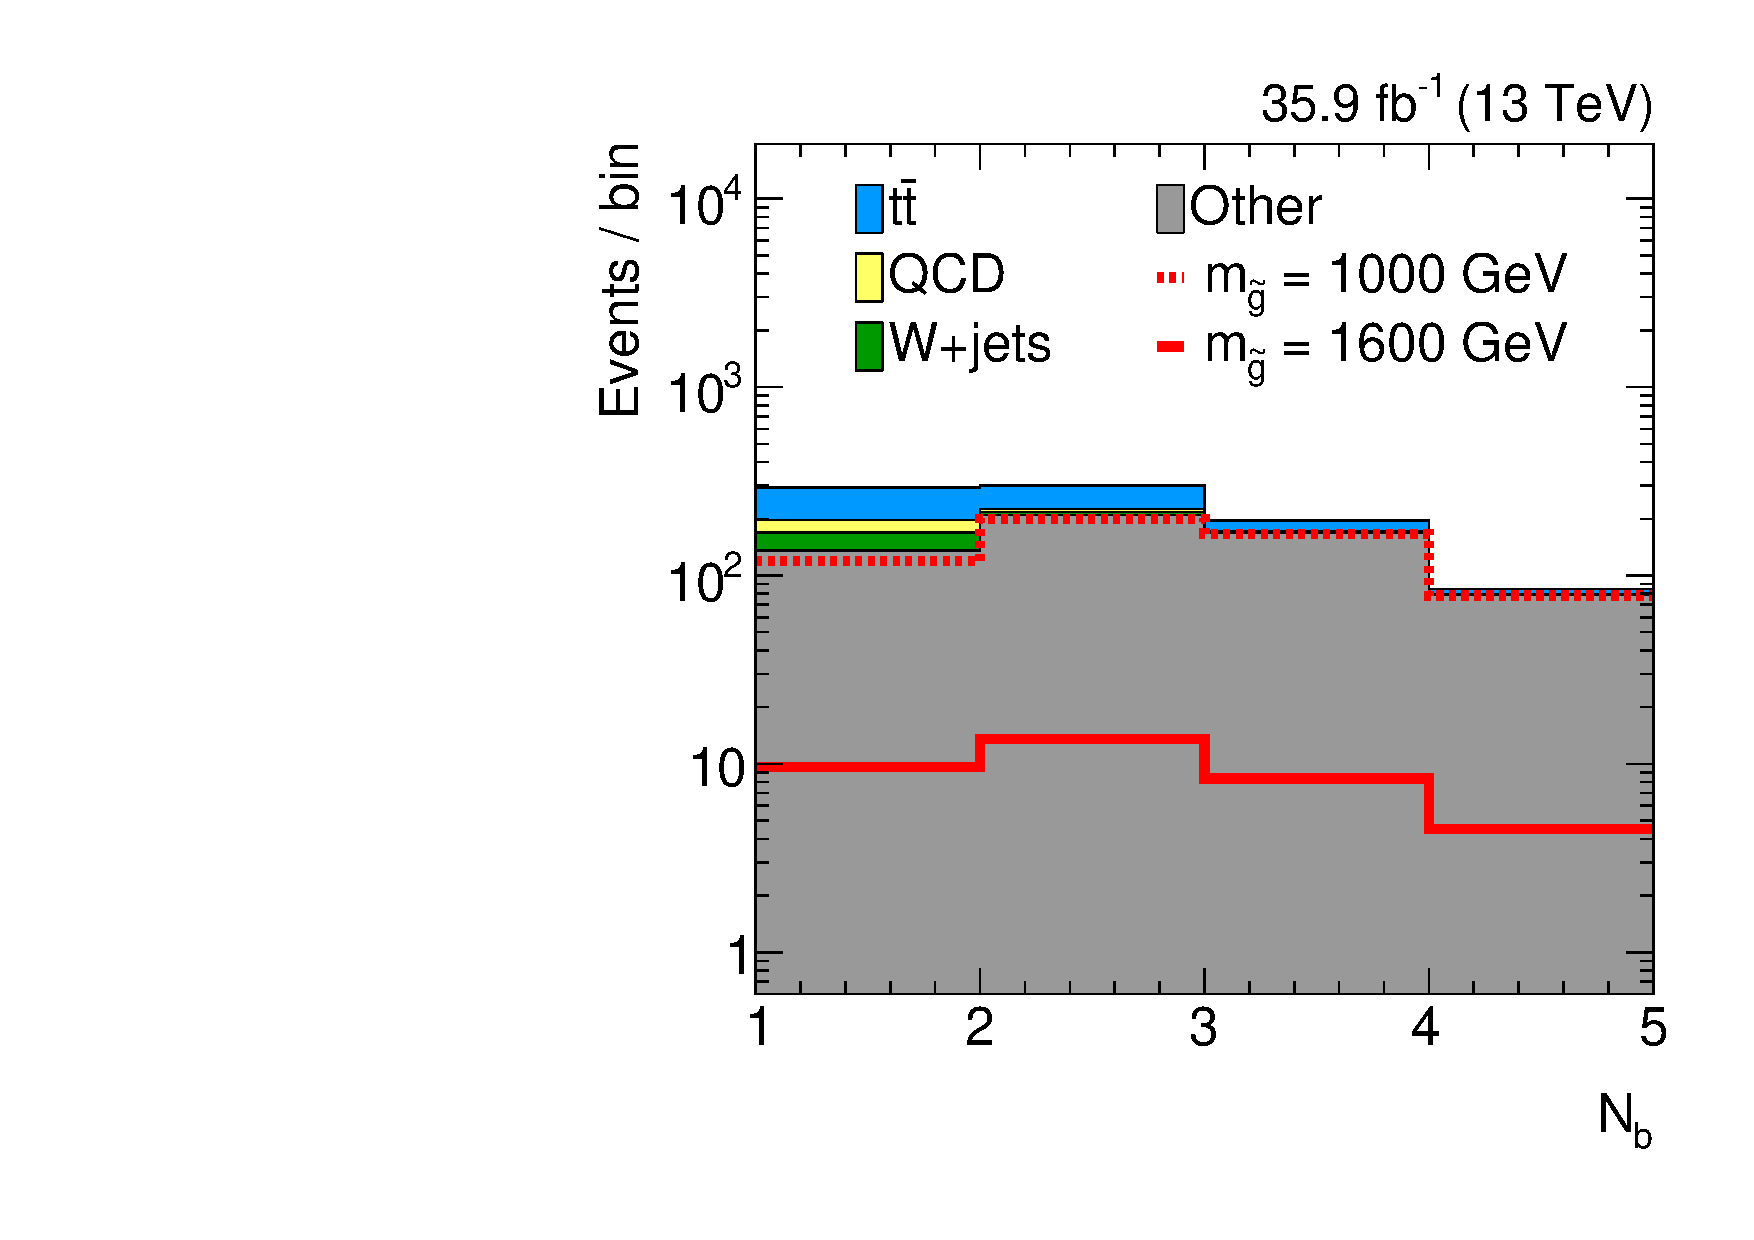
\includegraphics[angle=0,width=0.35\columnwidth]{fig/nb_nlep1_nj8_highmj.pdf}
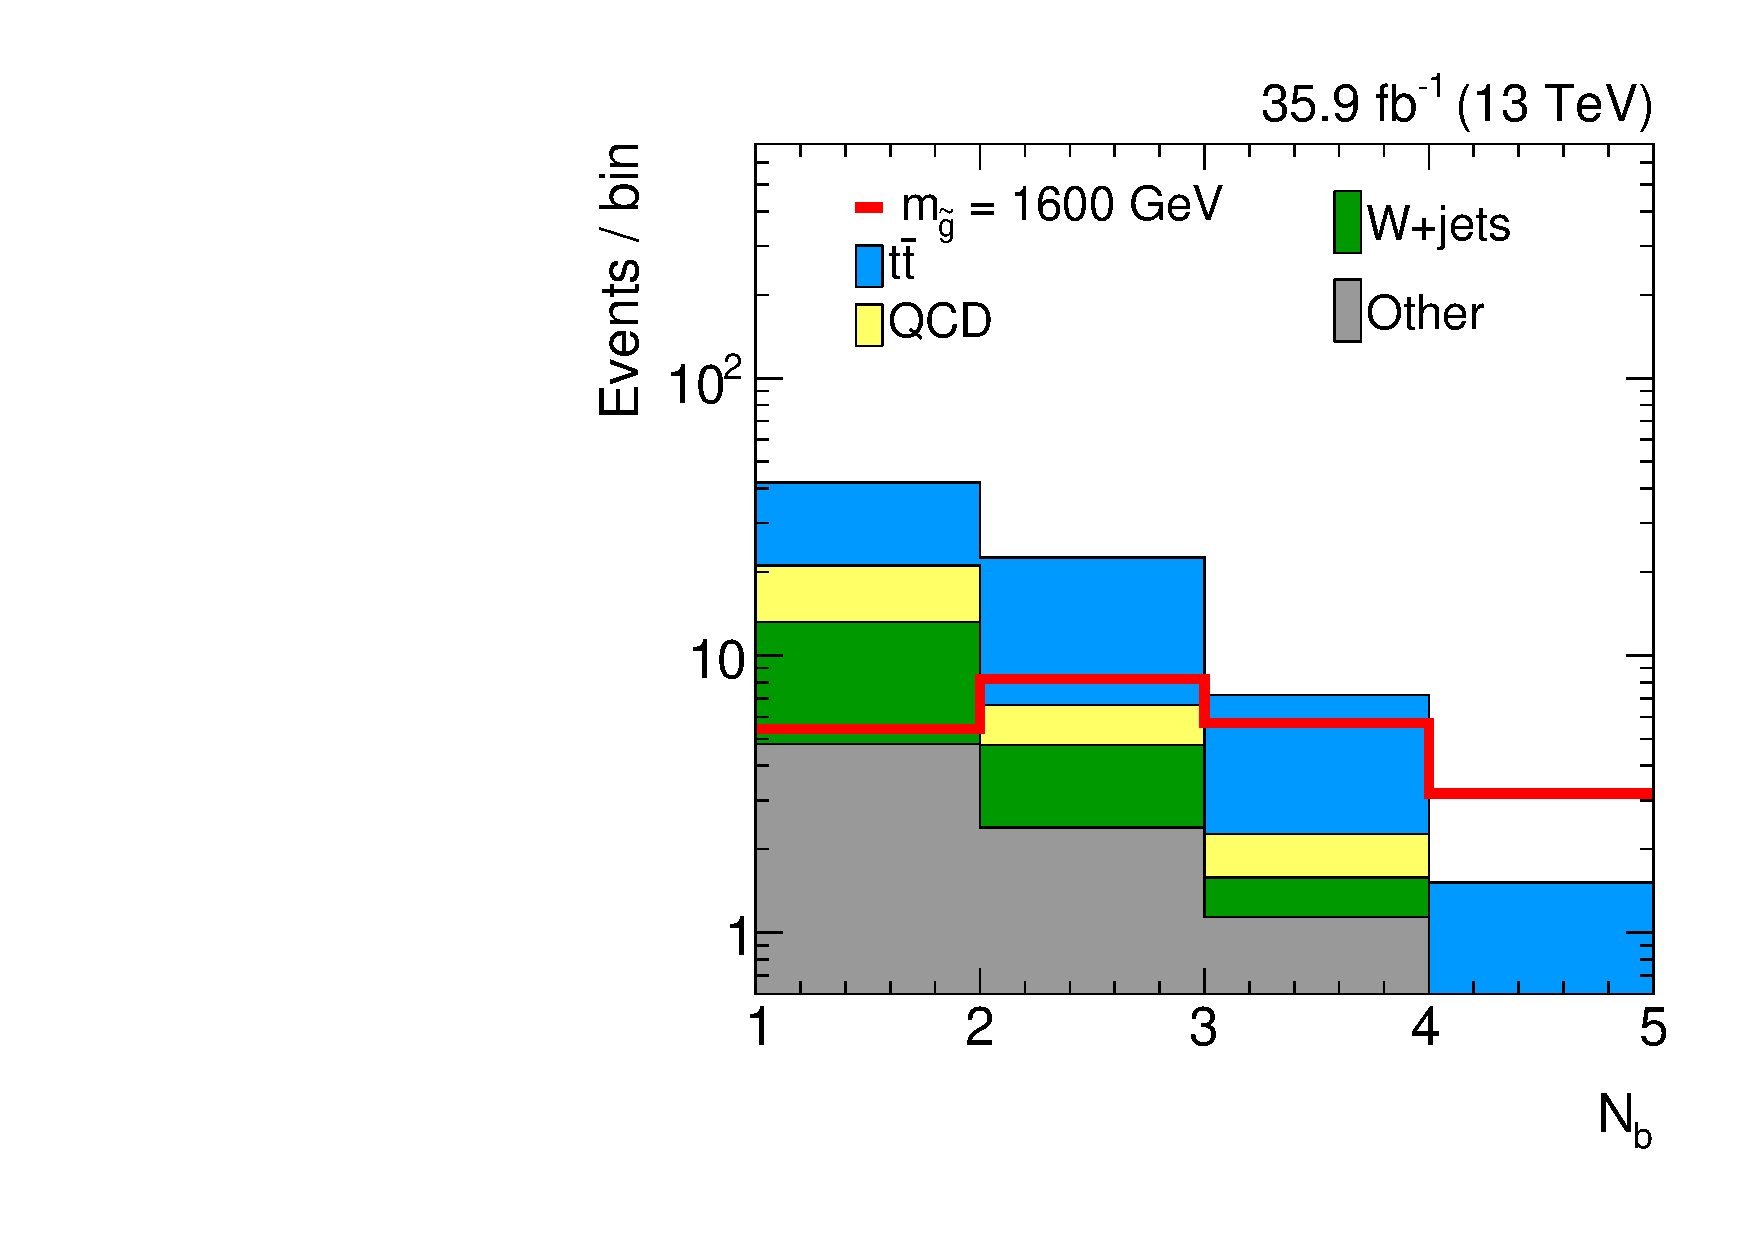
\includegraphics[angle=0,width=0.35\columnwidth]{fig/nb_nlep1_nj8_vhighmj.pdf}
\caption{The simulated \Nb distribution for background and signal processes in the signal region bins.
The top-left plot corresponds to the $6 \leq \Njets \leq 7$, $800 \leq \MJ \leq 1000~\GeV$ bin, the top-right plot to the $6 \geq \Njets \geq 7$, $\MJ \geq 1000~\GeV$ bin, the middle-left plot to the $\Njets \geq 8$, $500 \leq \MJ \leq 800~\GeV$ bin, the middle-right plot to the $\Njets \geq 8$, $800 \leq \MJ \leq 1000~\GeV$, and the bottom plot to the $\Njets \geq 8$, $\MJ \geq 1000~\GeV$ bin.}
\label{fig:nb_sr_dists}
\end{figure}

\end{section}
